%%%%%%%%%%%%%%%%%%%%%%%%%%%%%%%%%%%%%%%%%%%%%%%%%%%%%%%%%%%%%%%%%%%%%%
% Template for a UBC-compliant dissertation
% At the minimum, you will need to change the information found
% after the "Document meta-data"
%
%!TEX TS-program = pdflatex
%!TEX encoding = UTF-8 Unicode

%% The ubcdiss class provides several options:
%%   gpscopy (aka fogscopy)
%%       set parameters to exactly how GPS specifies
%%         * single-sided
%%         * page-numbering starts from title page
%%         * the lists of figures and tables have each entry prefixed
%%           with 'Figure' or 'Table'
%%       This can be tested by `\ifgpscopy ... \else ... \fi'
%%   10pt, 11pt, 12pt
%%       set default font size
%%   oneside, twoside
%%       whether to format for single-sided or double-sided printing
%%   balanced
%%       when double-sided, ensure page content is centred
%%       rather than slightly offset (the default)
%%   singlespacing, onehalfspacing, doublespacing
%%       set default inter-line text spacing; the ubcdiss class
%%       provides \textspacing to revert to this configured spacing
%%   draft
%%       disable more intensive processing, such as including
%%       graphics, etc.
%%

% For submission to GPS
\documentclass[gpscopy,onehalfspacing,11pt]{ubcdiss}

% For your own copies (looks nicer)
% \documentclass[balanced,twoside,11pt]{ubcdiss}

%%%%%%%%%%%%%%%%%%%%%%%%%%%%%%%%%%%%%%%%%%%%%%%%%%%%%%%%%%%%%%%%%%%%%%
%%%%%%%%%%%%%%%%%%%%%%%%%%%%%%%%%%%%%%%%%%%%%%%%%%%%%%%%%%%%%%%%%%%%%%
%%
%% FONTS:
%% 
%% The defaults below configures Times Roman for the serif font,
%% Helvetica for the sans serif font, and Courier for the
%% typewriter-style font.  Configuring fonts can be time
%% consuming; we recommend skipping to END FONTS!
%% 
%% If you're feeling brave, have lots of time, and wish to use one
%% your platform's native fonts, see the commented out bits below for
%% XeTeX/XeLaTeX.  This is not for the faint at heart. 
%% (And shouldn't you be writing? :-)
%%

%% NFSS font specification (New Font Selection Scheme)
\usepackage{times,mathptmx,courier}
\usepackage[scaled=.92]{helvet}

%% Math or theory people may want to include the handy AMS macros
\usepackage{amssymb}
\usepackage{amsmath}
\usepackage{amsfonts}

%% The pifont package provides access to the elements in the dingbat font.   
%% Use \ding{##} for a particular dingbat (see p7 of psnfss2e.pdf)
%%   Useful:
%%     51,52 different forms of a checkmark
%%     54,55,56 different forms of a cross (saltyre)
%%     172-181 are 1-10 in open circle (serif)
%%     182-191 are 1-10 black circle (serif)
%%     192-201 are 1-10 in open circle (sans serif)
%%     202-211 are 1-10 in black circle (sans serif)
%% \begin{dinglist}{##}\item... or dingautolist (which auto-increments)
%% to create a bullet list with the provided character.
\usepackage{pifont}

%%%%%%%%%%%%%%%%%%%%%%%%%%%%%%%%%%%%%%%%%%%%%%%%%%%%%%%%%%%%%%%%%%%%%%
%% Configure fonts for XeTeX / XeLaTeX using the fontspec package.
%% Be sure to check out the fontspec documentation.
%\usepackage{fontspec,xltxtra,xunicode}	% required
%\defaultfontfeatures{Mapping=tex-text}	% recommended
%% Minion Pro and Myriad Pro are shipped with some versions of
%% Adobe Reader.  Adobe representatives have commented that these
%% fonts can be used outside of Adobe Reader.
%\setromanfont[Numbers=OldStyle]{Minion Pro}
%\setsansfont[Numbers=OldStyle,Scale=MatchLowercase]{Myriad Pro}
%\setmonofont[Scale=MatchLowercase]{Andale Mono}

%% Other alternatives:
%\setromanfont[Mapping=tex-text]{Adobe Caslon}
%\setsansfont[Scale=MatchLowercase]{Gill Sans}
%\setsansfont[Scale=MatchLowercase,Mapping=tex-text]{Futura}
%\setmonofont[Scale=MatchLowercase]{Andale Mono}
%\newfontfamily{\SYM}[Scale=0.9]{Zapf Dingbats}
%% END FONTS
%%%%%%%%%%%%%%%%%%%%%%%%%%%%%%%%%%%%%%%%%%%%%%%%%%%%%%%%%%%%%%%%%%%%%%
%%%%%%%%%%%%%%%%%%%%%%%%%%%%%%%%%%%%%%%%%%%%%%%%%%%%%%%%%%%%%%%%%%%%%%



%%%%%%%%%%%%%%%%%%%%%%%%%%%%%%%%%%%%%%%%%%%%%%%%%%%%%%%%%%%%%%%%%%%%%%
%%%%%%%%%%%%%%%%%%%%%%%%%%%%%%%%%%%%%%%%%%%%%%%%%%%%%%%%%%%%%%%%%%%%%%
%%
%% Recommended packages
%%
\usepackage{texmf/checkend}	% better error messages on left-open environments
\usepackage{graphicx}	% for incorporating external images
%\graphicspath{{images}}
\usepackage{texmf/placeins}


%% booktabs: provides some special commands for typesetting tables as used
%% in excellent journals.  Ignore the examples in the Lamport book!
\usepackage{booktabs}

%% listings: useful support for including source code listings, with
%% optional special keyword formatting.  The \lstset{} causes
%% the text to be typeset in a smaller sans serif font, with
%% proportional spacing.
\usepackage{listings}
\lstset{basicstyle=\sffamily\scriptsize,showstringspaces=false,fontadjust}

%% The acronym package provides support for defining acronyms, providing
%% their expansion when first used, and building glossaries.  See the
%% example in glossary.tex and the example usage throughout the example
%% document.
%% NOTE: to use \MakeTextLowercase in the \acsfont command below,
%%   we *must* use the `nohyperlinks' option -- it causes errors with
%%   hyperref otherwise.  See Section 5.2 in the ``LaTeX 2e for Class
%%   and Package Writers Guide'' (clsguide.pdf) for details.
\usepackage[printonlyused,nohyperlinks]{texmf/acronym}
%% The ubcdiss.cls loads the `textcase' package which provides commands
%% for upper-casing and lower-casing text.  The following causes
%% the acronym package to typeset acronyms in small-caps
%% as recommended by Bringhurst.
\renewcommand{\acsfont}[1]{{\scshape \MakeTextLowercase{#1}}}

%% color: add support for expressing colour models.  Grey can be used
%% to great effect to emphasize other parts of a graphic or text.
%% For an excellent set of examples, see Tufte's "Visual Display of
%% Quantitative Information" or "Envisioning Information".
\usepackage{color}
\definecolor{greytext}{gray}{0.5}

%% comment: provides a new {comment} environment: all text inside the
%% environment is ignored.
%%   \begin{comment} ignored text ... \end{comment}
\usepackage{texmf/comment}

%% The natbib package provides more sophisticated citing commands
%% such as \citeauthor{} to provide the author names of a work,
%% \citet{} to produce an author-and-reference citation,
%% \citep{} to produce a parenthetical citation.
%% We use \citeeg{} to provide examples
\usepackage{natbib}
\newcommand{\citeeg}[1]{\citep[e.g.,][]{#1}}

%% The titlesec package provides commands to vary how chapter and
%% section titles are typeset.  The following uses more compact
%% spacings above and below the title.  The titleformat that follow
%% ensure chapter/section titles are set in singlespace.
\usepackage[compact]{texmf/titlesec}
\titleformat*{\section}{\singlespacing\raggedright\bfseries\Large}
\titleformat*{\subsection}{\singlespacing\raggedright\bfseries\large}
\titleformat*{\subsubsection}{\singlespacing\raggedright\bfseries}
\titleformat*{\paragraph}{\singlespacing\raggedright\itshape}

%% The caption package provides support for varying how table and
%% figure captions are typeset.
\usepackage[format=hang,indention=-1cm,labelfont={bf},margin=1em]{caption}

%% url: for typesetting URLs and smart(er) hyphenation.
%% \url{http://...} 
\usepackage{url}
\urlstyle{sf}	% typeset urls in sans-serif


%%%%%%%%%%%%%%%%%%%%%%%%%%%%%%%%%%%%%%%%%%%%%%%%%%%%%%%%%%%%%%%%%%%%%%
%%%%%%%%%%%%%%%%%%%%%%%%%%%%%%%%%%%%%%%%%%%%%%%%%%%%%%%%%%%%%%%%%%%%%%
%%
%% Possibly useful packages: you may need to explicitly install
%% these from CTAN if they aren't part of your distribution;
%% teTeX seems to ship with a smaller base than MikTeX and MacTeX.
%%
%\usepackage{pdfpages}	% insert pages from other PDF files
%\usepackage{longtable}	% provide tables spanning multiple pages
%\usepackage{chngpage}	% support changing the page widths on demand
%\usepackage{tabularx}	% an enhanced tabular environment

%% enumitem: support pausing and resuming enumerate environments.
%\usepackage{enumitem}

%% rotating: provides two environments, sidewaystable and sidewaysfigure,
%% for typesetting tables and figures in landscape mode.  
%\usepackage{rotating}

%% subfig: provides for including subfigures within a figure,
%% and includes being able to separately reference the subfigures.
%\usepackage{subfig}

%% ragged2e: provides several new new commands \Centering, \RaggedLeft,
%% \RaggedRight and \justifying and new environments Center, FlushLeft,
%% FlushRight and justify, which set ragged text and are easily
%% configurable to allow hyphenation.
%\usepackage{ragged2e}

%% The ulem package provides a \sout{} for striking out text and
%% \xout for crossing out text.  The normalem and normalbf are
%% necessary as the package messes with the emphasis and bold fonts
%% otherwise.
%\usepackage[normalem,normalbf]{ulem}    % for \sout

%%%%%%%%%%%%%%%%%%%%%%%%%%%%%%%%%%%%%%%%%%%%%%%%%%%%%%%%%%%%%%%%%%%%%%
%% HYPERREF:
%% The hyperref package provides for embedding hyperlinks into your
%% document.  By default the table of contents, references, citations,
%% and footnotes are hyperlinked.
%%
%% Hyperref provides a very handy command for doing cross-references:
%% \autoref{}.  This is similar to \ref{} and \pageref{} except that
%% it automagically puts in the *type* of reference.  For example,
%% referencing a figure's label will put the text `Figure 3.4'.
%% And the text will be hyperlinked to the appropriate place in the
%% document.
%%
%% Generally hyperref should appear after most other packages

%% The following puts hyperlinks in very faint grey boxes.
%% The `pagebackref' causes the references in the bibliography to have
%% back-references to the citing page; `backref' puts the citing section
%% number.  See further below for other examples of using hyperref.
%% 2009/12/09: now use `linktocpage' (Jacek Kisynski): GPS now prefers
%%   that the ToC, LoF, LoT place the hyperlink on the page number,
%%   rather than the entry text.
\usepackage[bookmarks,bookmarksnumbered,%
    allbordercolors={0.8 0.8 0.8},%
    pagebackref,linktocpage%
    ]{hyperref}
%% The following change how the the back-references text is typeset in a
%% bibliography when `backref' or `pagebackref' are used
\renewcommand\backrefpagesname{\(\rightarrow\) pages}
\renewcommand\backref{\textcolor{greytext} \backrefpagesname\ }

%% The following uses most defaults, which causes hyperlinks to be
%% surrounded by colourful boxes; the colours are only visible in
%% PDFs and don't show up when printed:
%\usepackage[bookmarks,bookmarksnumbered]{hyperref}

%% The following disables the colourful boxes around hyperlinks.
%\usepackage[bookmarks,bookmarksnumbered,pdfborder={0 0 0}]{hyperref}

%% The following disables all hyperlinking, but still enabled use of
%% \autoref{}
%\usepackage[draft]{hyperref}

%% The following commands causes chapter and section references to
%% uppercase the part name.
\renewcommand{\chapterautorefname}{Chapter}
\renewcommand{\sectionautorefname}{Section}
\renewcommand{\subsectionautorefname}{Section}
\renewcommand{\subsubsectionautorefname}{Section}

%% new command for the GIF manual style of table
\definecolor{GIFblue}{rgb}{0,0,0.6}
\newenvironment{fileExample}{
\begin{table}[h]
\color{GIFblue}
\ttfamily
}{\end{table} \color{black} \vspace{.1cm} }

\usepackage{gensymb}
%% If you have long page numbers (e.g., roman numbers in the 
%% preliminary pages for page 28 = xxviii), you might need to
%% uncomment the following and tweak the \@pnumwidth length
%% (default: 1.55em).  See the tocloft documentation at
%% http://www.ctan.org/tex-archive/macros/latex/contrib/tocloft/
% \makeatletter
% \renewcommand{\@pnumwidth}{3em}
% \makeatother

%%%%%%%%%%%%%%%%%%%%%%%%%%%%%%%%%%%%%%%%%%%%%%%%%%%%%%%%%%%%%%%%%%%%%%
%%%%%%%%%%%%%%%%%%%%%%%%%%%%%%%%%%%%%%%%%%%%%%%%%%%%%%%%%%%%%%%%%%%%%%
%%
%% Some special settings that controls how text is typeset
%%
% \raggedbottom		% pages don't have to line up nicely on the last line
% \sloppy		% be a bit more relaxed in inter-word spacing
% \clubpenalty=10000	% try harder to avoid orphans
% \widowpenalty=10000	% try harder to avoid widows
% \tolerance=1000

%% And include some of our own useful macros
% This file provides examples of some useful macros for typesetting
% dissertations.  None of the macros defined here are necessary beyond
% for the template documentation, so feel free to change, remove, and add
% your own definitions.
%
% We recommend that you define macros to separate the semantics
% of the things you write from how they are presented.  For example,
% you'll see definitions below for a macro \file{}: by using
% \file{} consistently in the text, we can change how filenames
% are typeset simply by changing the definition of \file{} in
% this file.
% 
%% The following is a directive for TeXShop to indicate the main file
%%!TEX root = diss.tex

\newcommand{\NA}{\textsc{n/a}}	% for "not applicable"
\newcommand{\eg}{e.g.,\ }	% proper form of examples (\eg a, b, c)
\newcommand{\ie}{i.e.,\ }	% proper form for that is (\ie a, b, c)
\newcommand{\etal}{\emph{et al}}

% Some useful macros for typesetting terms.
\newcommand{\file}[1]{\texttt{#1}}
\newcommand{\class}[1]{\texttt{#1}}
\newcommand{\latexpackage}[1]{\href{http://www.ctan.org/macros/latex/contrib/#1}{\texttt{#1}}}
\newcommand{\latexmiscpackage}[1]{\href{http://www.ctan.org/macros/latex/contrib/misc/#1.sty}{\texttt{#1}}}
\newcommand{\env}[1]{\texttt{#1}}
\newcommand{\BibTeX}{Bib\TeX}

% Define a command \doi{} to typeset a digital object identifier (DOI).
% Note: if the following definition raise an error, then you likely
% have an ancient version of url.sty.  Either find a more recent version
% (3.1 or later work fine) and simply copy it into this directory,  or
% comment out the following two lines and uncomment the third.
\DeclareUrlCommand\DOI{}
\newcommand{\doi}[1]{\href{http://dx.doi.org/#1}{\DOI{doi:#1}}}
%\newcommand{\doi}[1]{\href{http://dx.doi.org/#1}{doi:#1}}

% Useful macro to reference an online document with a hyperlink
% as well with the URL explicitly listed in a footnote
% #1: the URL
% #2: the anchoring text
\newcommand{\webref}[2]{\href{#1}{#2}\footnote{\url{#1}}}

% epigraph is a nice environment for typesetting quotations
\makeatletter
\newenvironment{epigraph}{%
	\begin{flushright}
	\begin{minipage}{\columnwidth-0.75in}
	\begin{flushright}
	\@ifundefined{singlespacing}{}{\singlespacing}%
    }{
	\end{flushright}
	\end{minipage}
	\end{flushright}}
\makeatother

% \FIXME{} is a useful macro for noting things needing to be changed.
% The following definition will also output a warning to the console
\newcommand{\FIXME}[1]{\typeout{**FIXME** #1}\textbf{[FIXME: #1]}}

% END


%%%%%%%%%%%%%%%%%%%%%%%%%%%%%%%%%%%%%%%%%%%%%%%%%%%%%%%%%%%%%%%%%%%%%%
%%%%%%%%%%%%%%%%%%%%%%%%%%%%%%%%%%%%%%%%%%%%%%%%%%%%%%%%%%%%%%%%%%%%%%
%%
%% Document meta-data: be sure to also change the \hypersetup information
%%

\title{Geological and Petrophysical Information in Geophysical Inversion Problems}
\subtitle{DRAFT: \today}

\author{Daniel Bild-Enkin}
\previousdegree{BSc Honours, The University of Toronto, 2012}

% What is this dissertation for?
\degreetitle{Masters of Science}

\institution{The University of British Columbia}
\campus{Vancouver}

\faculty{THE FACULTY OF GRADUATE AND POSTDOCTORAL
STUDIES}
\department{Geophysics}
\submissionmonth{August}
\submissionyear{2016}

%% hyperref package provides support for embedding meta-data in .PDF
%% files
\hypersetup{
  pdftitle={DBE thesis  (DRAFT: \today)},
  pdfauthor={Daniel Bild-Enkin},
  pdfkeywords={}
}

%%%%%%%%%%%%%%%%%%%%%%%%%%%%%%%%%%%%%%%%%%%%%%%%%%%%%%%%%%%%%%%%%%%%%%
%%%%%%%%%%%%%%%%%%%%%%%%%%%%%%%%%%%%%%%%%%%%%%%%%%%%%%%%%%%%%%%%%%%%%%
%% 
%% The document content
%%

%% LaTeX's \includeonly commands causes any uses of \include{} to only
%% include files that are in the list.  This is helpful to produce
%% subsets of your thesis (e.g., for committee members who want to see
%% the dissertation chapter by chapter).  It also saves time by 
%% avoiding reprocessing the entire file.
%\includeonly{intro,conclusions}
%\includeonly{discussion}

\begin{document}

%%%%%%%%%%%%%%%%%%%%%%%%%%%%%%%%%%%%%%%%%%%%%%%%%%
%% From Thesis Components: Tradtional Thesis
%% <http://www.grad.ubc.ca/current-students/dissertation-thesis-preparation/order-components>

% Preliminary Pages (numbered in lower case Roman numerals)
%    1. Title page (mandatory)
\maketitle

%    2. Abstract (mandatory - maximum 350 words)
%% The following is a directive for TeXShop to indicate the main file
%%!TEX root = diss.tex

\chapter{Abstract}

This document provides brief instructions for using the \class{ubcdiss}
class to write a \acs{UBC}-conformant dissertation in \LaTeX.  This
document is itself written using the \class{ubcdiss} class and is
intended to serve as an example of writing a dissertation in \LaTeX.
This document has embedded \acp{URL} and is intended to be viewed
using a computer-based \ac{PDF} reader.

Note: Abstracts should generally try to avoid using acronyms.

Note: at \ac{UBC}, both the \ac{GPS} Ph.D. defence programme and the
Library's online submission system restricts abstracts to 350
words.

% Consider placing version information if you circulate multiple drafts
%\vfill
%\begin{center}
%\begin{sf}
%\fbox{Revision: \today}
%\end{sf}
%\end{center}

\cleardoublepage

%    3. Preface
%% The following is a directive for TeXShop to indicate the main file
%%!TEX root = diss.tex

\chapter{Preface}


\cleardoublepage

%    4. Table of contents (mandatory - list all items in the preliminary pages
%    starting with the abstract, followed by chapter headings and
%    subheadings, bibliographies and appendices)
\tableofcontents
\cleardoublepage	% required by tocloft package

%    5. List of tables (mandatory if thesis has tables)
\listoftables
\cleardoublepage	% required by tocloft package

%    6. List of figures (mandatory if thesis has figures)
\listoffigures
\cleardoublepage	% required by tocloft package

%    7. List of illustrations (mandatory if thesis has illustrations)
%    8. Lists of symbols, abbreviations or other (optional)

%    9. Glossary (optional)
%% The following is a directive for TeXShop to indicate the main file
%%!TEX root = diss.tex

\chapter{Glossary}

This glossary uses the handy \latexpackage{acroynym} package to automatically
maintain the glossary.  It uses the package's \texttt{printonlyused}
option to include only those acronyms explicitly referenced in the
\LaTeX\ source.

% use \acrodef to define an acronym, but no listing
\acrodef{UI}{user interface}
\acrodef{UBC}{University of British Columbia}

% The acronym environment will typeset only those acronyms that were
% *actually used* in the course of the document
\begin{acronym}[ANOVA]
\acro{ANOVA}[ANOVA]{Analysis of Variance\acroextra{, a set of
  statistical techniques to identify sources of variability between groups}}
\acro{API}{application programming interface}
\acro{CTAN}{\acroextra{The }Common \TeX\ Archive Network}
\acro{DOI}{Document Object Identifier\acroextra{ (see
    \url{http://doi.org})}}
\acro{GPS}[GPS]{Graduate and Postdoctoral Studies}
\acro{PDF}{Portable Document Format}
\acro{RCS}[RCS]{Revision control system\acroextra{, a software
    tool for tracking changes to a set of files}}
\acro{TLX}[TLX]{Task Load Index\acroextra{, an instrument for gauging
  the subjective mental workload experienced by a human in performing
  a task}}
\acro{UML}{Unified Modelling Language\acroextra{, a visual language
    for modelling the structure of software artefacts}}
\acro{URL}{Unique Resource Locator\acroextra{, used to describe a
    means for obtaining some resource on the world wide web}}
\acro{W3C}[W3C]{\acroextra{the }World Wide Web Consortium\acroextra{,
    the standards body for web technologies}}
\acro{XML}{Extensible Markup Language}
\end{acronym}

% You can also use \newacro{}{} to only define acronyms
% but without explictly creating a glossary
% 
% \newacro{ANOVA}[ANOVA]{Analysis of Variance\acroextra{, a set of
%   statistical techniques to identify sources of variability between groups.}}
% \newacro{API}[API]{application programming interface}
% \newacro{GOMS}[GOMS]{Goals, Operators, Methods, and Selection\acroextra{,
%   a framework for usability analysis.}}
% \newacro{TLX}[TLX]{Task Load Index\acroextra{, an instrument for gauging
%   the subjective mental workload experienced by a human in performing
%   a task.}}
% \newacro{UI}[UI]{user interface}
% \newacro{UML}[UML]{Unified Modelling Language}
% \newacro{W3C}[W3C]{World Wide Web Consortium}
% \newacro{XML}[XML]{Extensible Markup Language}
	% always input, since other macros may rely on it

\textspacing		% begin one-half or double spacing

%   10. Acknowledgements (optional)
%% The following is a directive for TeXShop to indicate the main file
%%!TEX root = diss.tex

\chapter{Acknowledgments}

Thank those people who helped you. 

Don't forget your parents or loved ones.

You may wish to acknowledge your funding sources.


%   11. Dedication (optional)

% Body of Thesis (not all sections may apply)
\mainmatter

\acresetall	% reset all acronyms used so far

%    1. Introduction
%% The following is a directive for TeXShop to indicate the main file
%%!TEX root = diss.tex

\chapter{Introduction}
\label{ch:Introduction}

\begin{epigraph}
\emph{The 'true' is only the expedient in our way of thinking, just as the 'right' is only the expedient in our way of behaving.}\\
---~William James (1909)
\end{epigraph}


In all cases these are first guesses at what needs to be in each section more or less detail need to be added.


\section{What problems}
\label{sec:What problems}

Geophysical inversions, specifically potential fields 
include formulation of non-regularized inverse problem

\section{Difficulties with said problems }
\label{sec:Difficulties with said problems }

The standard way to fit a set of parameters to a set of data (especially when they are related by a linear operator) is least squares optimization. This is rendered problematic since, in general, geo-physical inversions are ill-conditioned (define) and undetermined (define) (\cite{oldenburg2005inversion} other sources I'm sure). In specific potential fields are particularly under-determined due to the lack of any depth information in the data.

show some form of problems with forward operator matrix in PF inversion

\section{Solutions to said difficulties}
\label{sec:Solutions to said difficulties}

To mitigate the difficulties presented above an extra term is added to the optimization. 

\begin{align}
\phi = \phi_d + \beta\phi_m
\end{align}
\label{eq:objective function}

where $\phi_m$ is called the \ac{MOF} or model norm. This $\phi_m$ can be defined in many ways, following  \cite{oldenburg2005inversion}

\begin{align}
\phi_m(m) &= \alpha_s\int(m-m_{ref})^2dx+\alpha_x\int\bigg(\frac{d}{dx}(m-m_{ref})\bigg)^2dx\\
&=\alpha_s\|\textbf{W}_s(m-m_{ref})\|^2_2+\alpha_x\|\textbf{W}_x(m-m_{ref})\|^2_2
\end{align}
\label{eq:MOF}

in higher dimensions more smoothness terms can be added. The $\textbf{W}$ terms contain both the operator (identity for $\textbf{W}_s$ and derivative for $\textbf{W}_x$ and other dimensions) and the relative weight each cell or face contributes to the \ac{MOF}. This gives us several levers to add a-priori information into the inversion.

The \ac{MOF} allows us to mathematically solve the problem by adding a priori information into the inversion. Namely we assume that the recovered model should be small and smooth. There are times when this is desired but often we have more specific information about the true model that needs to be inserted into the inversion. Luckily the various terms in the \ac{MOF} allow us to add a significant amount of information is various ways to the inversion.
	It must be said that all of the techniques listed below are not novel. Many researchers before me have used exactly these techniques to constrain inversions (\cite{williams2008geologicall},\cite{Lelievre2009Integrating} among other (still need to add more)). What is novel in this thesis is the creation of a suit of tools (created by me and the rest of the GIF group) to make the incorporation of geological data into the \ac{MOF} of inversions easy even in non-trivial cases.

\subsection{$\alpha$ coefficients}
\label{sec:alpha coefficients}

broad strokes weights the relative importance of the smallness and smoothness in the various directions. can also be thought of as length scales

\subsection{Reference Models}
\label{sec:Reference Models}

we don't always want a model to be close to zero. Sometimes it should be close to another constant sometimes we have guesses of the property in some places and want the inversion result to be close to that value

\subsection{Weighting matrices}
\label{sec:Weighting matrices}

much more precise. Can put interfaces in precise locations. Can also force a model towards the reference model where we are more sure
\\\\
along with the terms in the \ac{MOF} other parts of the optimization algorithm (may need more info in the optimization) can be used to add information into the inversion

\subsection{Initial Model}
\label{sec:Initial Model}

In the optimization we assume that the initial guess is near enough to the truth that the problem is locally convex. The initial model is important in that way. In an under determined system it also provides a way to push the inversion towards a given result. Often the initial model is simply the reference model, or the reference model shifted slightly to keep it within the bounds

\subsection{Bounds}
\label{sec:Bounds}

we can also set values that each cell of the final model must lie between. This allows for a hard setting of confidence intervals in the physical properties

\subsection{$L_p L_q$ weights}
\label{sec:Lp Lq weights}

Finally we can generalize the \ac{MOF} somewhat. In \autoref{eq:MOF} we used $L_2$ norms as this is a natural norm that promotes a smoothly varying model that is close to the reference model. We do not always want such a model and can change the norm used in the \ac{MOF}. Lower norms promote more sparsity in whatever measure they are being applied to. This leads to models being more compact (should lowever norms be applied to the smallness term) or more blocky with greater discontinuities (should lower norms be applied to one or more smoothness terms). Non $L_2$ norms can be applied across the whole \ac{MOF} or can be applied variably across the model. This allows for placing discontinuities in a given direction but not perfectly placing the location allowing the inversion algorithm more freedom to chose the location itself.

\section{Forms of A Priori Information}
\label{sec:Forms of A Priori Information}

\subsection{Bore Hole Data and the Use of Koenigsberger Ratios to Correct Bore Hole Susceptibility Measurements}
\label{sec: Bore Hole Data}

Bore holes provide physical property measurements at depth either by sending geophysical instruments down hole or by recovering a core and then measuring it subsequently in the lab. Bore holes can also provide qualitative rock unit information. Much work has been done on including physical property bore hole information(\cite{williams2008geologically} among others I'm sure). If we can convert the lithology information from bore holes into physical property information (using petrophysical measurements of reasonably similar rocks) we can use the information in the same fashion as a physical property bore hole logs.

In some contexts one physical property can be used as a proxy for others. In one case study, we have magnetic susceptibility measurements down hole but surface samples have been measured which reveal high magnetic remanence. The simple susceptibility measurement is drastically lower than the recovered effective susceptibility derived from the inversion of a magnetic survey over the area. This is due to the fact that the inversion is recovering effective susceptibility (induced magnetization plus \ac{NRM} normalized by and assuming the direction of earth's field in the location). To describe the method we need to discuss the general derivation of the magnetostatic problem and then discuss the effects of \ac{NRM} on measured data and the recovered inversion result. 

The following derivation follows the one in \cite{fournier2015cooperative}. We can derive the magnetostatic problem from Maxwell's equations. If we assume no free currents and no time varying electric field Maxwell's equations simplify to 

\begin{equation} 
\label{eq:maxwellB}
\mathbf{\nabla} \cdot \mathbf{B} = 0\\
\end{equation}
\begin{equation}
\label{eq:maxwelH}
\mathbf{\nabla} \times \mathbf{H} = 0\\   
\end{equation}
\begin{equation}
\label{eq:maxwellHB}
\mathbf{B} = \mu\mathbf{H},
\end{equation}
where $\mathbf{B}$ is the magnetic flux density measured in Tesla (T), $\mathbf{H}$ is the magnetic field measured in amperes per meter (A/m), and $\mu$ is magnetic permeability which relates  $\mathbf{B}$ to $\mathbf{H}$ in matter. We can rewrite $\mu$ to take the permeability of free space ($\mu_0$) into account and state that
\begin{equation}\label{eq:susc}
\mu = \mu_0(1 + \kappa),
\end{equation}
where $\mu_0$ is the permeability of free space ($4\pi\times10^{-7}\frac{Tm}{A}$), and $\kappa$ is the magnetic susceptibility of a material. $\kappa$ is dimensionless and describes the ability of a material to become magnetized under some field $\mathbf{H}$. The definition of $\kappa$ in \autoref{eq:susc}  gives us a definition for induced magnetization
\begin{equation}\label{eq:Mi}
\mathbf M_I = \kappa\textbf{H}.
\end{equation}
Since there are no free currents and \autoref{eq:maxwelH} states that $\mathbf{H}$ has no curl, it can be written as the gradient of a potential field
\begin{equation}\label{eq:phi}
\mathbf{H} = \mathbf{\nabla}\phi.
\end{equation}
Since, by \autoref{eq:maxwellB}, we assume that there are no magnetic monopoles, we approximate $\phi$ in terms of a dipole moment $\mathbf m$. If we have a magnetic dipole with a moment of $\mathbf m$ at a location $\mathbf r_Q$, then the potential field $\phi$ as measured at some $\mathbf r_P$ is given by
\begin{equation}\label{eq:phiOfmDiscrete}
\phi(r) = \frac{1}{4\pi}\mathbf m\cdot \mathbf{\nabla}\Big(\frac{1}{r}\Big),
\end{equation}
where
\begin{equation}\label{eq:rDef}
\mathbf r = \| \mathbf r_Q - \mathbf r_P\|_2.
\end{equation}
We can generalize \autoref{eq:phiOfmDiscrete} to a continuous form by replacing the discrete $\mathbf m$ with a continuous $\mathbf M$ and integrating
\begin{equation}\label{eq:phiOfmCont}
\phi( r) = \frac{1}{4\pi}\int_V\mathbf M\cdot \mathbf{\nabla}\Big(\frac{1}{r}\Big)dv.
\end{equation}
If we take the gradient of \autoref{eq:phiOfmCont} we find $\mathbf B$ the magnetic flux density,\\\\
\begin{equation}\label{eq:BOfPcont}
\mathbf B (\mathbf r_P) = \frac{1}{4\pi}\int_V\mathbf M\cdot \mathbf{\nabla}\mathbf{\nabla}\Big(\frac{1}{r}\Big)dv.
\end{equation}
In \autoref{eq:BOfPcont} the dependency of $\mathbf B$ on $\mathbf r_P$ is due to the fact that $r$ depends on $\mathbf r_P$ as in \autoref{eq:rDef}. In most geophysical surveys, the full vector $\mathbf B$ is not collected, usually only its magnitude, or the \ac{TMI},
\begin{equation}\label{eq:TMI}
B_{TMI} = \| \mathbf B_0 + \mathbf B_A\|_2
\end{equation}
where $\mathbf B_0$ is the primary field (earth's field) and $\mathbf B_A$ is the anomalous local field due to magnetization in the ground. For the purposes of geophysical exploration we are only interested in $\mathbf B_A$. Since we are only interested in $\mathbf B_A$ a useful quantity is therefor the \ac{TMA}, defined as
\begin{equation}\label{eq:TMA}
B_{TMA} = \| \mathbf B_{Total} + \mathbf B_0\|_2
\end{equation}
\ac{TMA} is difficult to measure directly but can be approximated assuming $\frac{\|\mathbf B_A\|}{\|\mathbf B_0\|} \ll 1$,
\begin{align}\label{eq:TMAaprox}
B_{TMA} &\simeq \mathbf B_A\cdot \hat{\mathbf B}_0\\
&=\|\mathbf B_0+\mathbf B_A\| - \|\mathbf B_0\|
\end{align}
We now have a formulation of $\mathbf B$ that depends on magnetization $\mathbf M$, the vector field of magnetization in the ground and the quantities collected in geophysical magnetics surveys. We will now take a more specific look at magnetization and its effects both on $\mathbf B$ and $B_{TMA}$. If we assume no self-demagnetization (which is reasonable for susceptibilities below $1\time10^{-2}$ \cite{lelievre2006magnetic}) the inducing magnetic field is constant over the volume to be inverted and total magnetization can be characterized by the following
\begin{align} \label{eq:magnetization}
\textbf{M} &= \mathbf M_I + \textbf{M}_{NRM}\\
\textbf{M} &= \kappa\textbf{H} + \textbf{M}_{NRM}
\end{align}
Here $\textbf M$ is the total magnetization, $\mathbf M_I$ is the induced magnetization as in \autoref{eq:Mi} , $\kappa$ is susceptibility as defined in \autoref{eq:susc}, $\textbf{H}$ is the inducing field (in this case of the geomagnetic field) and $\textbf{M}_{NRM}$ is the \ac{NRM}. $\textbf{M}_{NRM}$  is also characterized by what is called Koenigsberger ratio
\begin{equation} \label{eq:Koenigsberger}
Q = \frac{\textbf{M}_{NRM}}{ \kappa\textbf{H}} = \frac{\text{remanent magnetization}}{\text{induced magnetization}}
\end{equation}
In the case where \ac{NRM} is negligible, the direction of $\mathbf M$ isthe same as $\mathbf H$, meaning that $\mathbf B_A$ and $\mathbf B_0$ are in the same direction and making the approximation in \autoref{eq:TMAaprox} exact. The methods outlined in \cite{li19963} and \cite{pilkington19973} assume that not only is there no self-demagnetization but also that there is no \ac{NRM}. A slight generalization from assuming no \ac{NRM} is that the anomalous magnetization is entirely in one direction \cite{li19963}. The recovered quantity is effective susceptibility, or magnetization normalized by the earth's field,
\begin{equation} \label{eq:effSusc}
\kappa_{eff} =  \frac{\|\mathbf M\|}{\|\mathbf H\|}.
\end{equation}In the case that the magnitude of \ac{NRM} is negligible, effective susceptibility and the true susceptibility are equal (i.e. $Q \ll 1)$.

	In the context of high remanent magnetization, the assumption that there is no \ac{NRM} is by definition clearly false and \ac{NRM} affects the inversion results. In the case that the \ac{NRM} is in a similar direction as the earth's field, the measured field $B_{TMA}$ will be higher than expected, given only susceptibility, and thus the recovered $\kappa_{eff}$ will be higher than the true $\kappa$. Similarly, in the case that \ac{NRM} is in a direction nearly anti-parallel to the earth's field, the measured field $B_{TMA}$ will be lower than expected, given only susceptibility, and thus the recovered $\kappa_{eff}$ will also be lower than the true $\kappa$.
	
	Understanding the difference between $\kappa$ and $\kappa_{eff}$ is very important with respect to inserting magnetic petrophysical measurements into an inversion's \ac{MOF}. It is an unfortunate truth that susceptibility is significantly easier to measure than \ac{NRM}. As stated above in \autoref{eq:susc} the permeability of an object is related to its susceptibility. In addition the inductance of a coil is proportional to the permeability inside and around it and thus is dependent on the susceptibility of the material. This change in inductance of a coil allows the precise measurement of susceptibility without contamination by \ac{NRM} \cite{collinson1983methods},\cite{clark1991notes}. The measurement of the inductance of a coil also allows the measurement of susceptibility of a rock without reorienting the sample and without shielding from ambient magnetic fields \cite{collinson1983methods}.
	
On the other hand, \ac{NRM} as opposed to susceptibility is a vector quantity and thus the sample must be reoriented to measure it from different directions, even when only the magnitude of the \ac{NRM} is required. In addition, unless the sample is very highly magnetized and stable, measurement will require shielding from ambient fields.

As can be seen from the above, it is not surprising that n the case of El Poma we have many susceptibility measurements including bore-holes and very few (only two within the areas of interest) measurements of \ac{NRM}. However, if susceptibility is used to constrain an inversion in an area of strong \ac{NRM} the inversion could be constrained to a value much higher or lower than the true effective susceptibility. 

At first order, a potential correction given \ac{NRM} measurements is to use the Koenigsberger ratio of a sample and assume that other samples will have a similar Koenigsberger ratio. It is recognized that this assumption will not be true. That said it is a closer approximation than would otherwise be possible without the sample. Once we have a Koenigsberger ratio and a susceptibility we can determine the magnetization of the sample using \autoref{eq:magnetization} and  \autoref{eq:Koenigsberger} in the form
\begin{equation} \label{eq:Qcorrection}
\textbf{M}_{eff} = \kappa\textbf{H} + \|Q\kappa\textbf{H}\|\hat{\mathbf M}_{NRM},
\end{equation}	
where $Q$ is the Koenigsberger ratio used and $\hat{\mathbf M}_{NRM}$ is the magnetization direction of the sample used. It is important to note that \autoref{eq:Qcorrection} is a vector sum and the direction of $\mathbf{M}_{eff}$ will not be in the direction of either $\mathbf H$ or $\mathbf M_{NRM}$. It is also interesting to note that \autoref{eq:Qcorrection} is more generally true if more samples have \ac{NRM} measurements. If, instead of being a single measurement, we have a more detailed estimate of each sample's Koenigsberger ratio and magnetization direction, we can get a better estimate of $\mathbf M_{eff}$.
	
\subsection{Surface Sample Data}
\label{sec: Surface Sample Data}

\subsection{Geological Maps}
\label{sec: Geological Maps}


\section{Using Multiple Data Types, with Clustering}
\label{sec:Using Multiple Data Types, with Clustering}


\endinput

 Interestingly, the assumption that all magnetizations are in the same direction also assumes that all Koenigsberger ratios are equal.

Any text after an \endinput is ignored.
You could put scraps here or things in progress.


%    2. Main body
% Generally recommended to put each chapter into a separate file
%\include{relatedwork}
%\include{model}
%\include{impl}
%\include{discussion}
%\include{conclusions}

%% The following is a directive for TeXShop to indicate the main file
%%!TEX root = diss.tex

\chapter{Tools for Integrating Geological and Petrophysical Information into the Regularization of Inversions}
\label{ch:GIFtools}

\section{Including Bore Hole Information in Inversion Regularization}
\label{sec:BHandSS}

Bore holes provide physical property measurements at depth either by providing a conduit to send geophysical instruments down hole or by recovering a core and then measuring its petrophysical properties subsequently in the lab.  The inversion methods for including physical property and lithology bore hole data  have been developed (e.g., \cite{williams2008geologically}). In this section I discuss how GIFtools and Model Builder incorporate bore hole information into inversion constraints in a expedient and effective manner.

In addition to physical property data, bore holes can also provide qualitative rock unit information. In this section I show the linking of lithology information from bore holes with physical property information using petrophysical measurements of reasonably similar rocks. Once this linking is done, the bore hole information can be used in the same fashion as a physical property bore hole logs.

In this section I also show the advantage of integrating the creation of inversion constraints with more general data processing tools. Once we have a set of sample data from either bore hole or surface samples loaded into GIFtools, we can then use the general data modification tools that are already provided for data quality control created both by me and the rest of the \ac{GIF} team.

\subsection{Importing Bore Hole Data}
\label{subsec:importBH}

Bore hole data is typically stored in three separate files: the collar file, the survey file, and the property file. The collar file contains the spacial information of the very top of the hole.  \autoref{tab:collarEx} shows an example collar file. GIFtools is sufficiently flexible that it can read both whitespace and comma delimited files. Additionally as long as there are headers for each column, it does not matter what order the columns appear in, as the correct columns for each purpose can be specified during the import process. Finally while the example shows a text hole identifier, it is also possible to identify individual holes by a numerical index.
\begin{fileExample}
\begin{tabular}{|ccccc|}   
\hline
\multicolumn{5}{|l|}{\% TKC collar data} \\
HOLE-ID & X & Y & Z & LENGTH \\
DO27-05-01 & 557187 & 7133758 & 418 & 58.52 \\
DO27-05-02 & 557191 & 7133755 & 418 & 459.5 \\
DO27-05-03 & 557165 & 7133682 & 418 & 230 \\
DO27-05-04 & 557425 & 7133835 & 420 & 112.5 \\
DO27-05-05 & 557425 & 7133835 & 420 & 99.8 \\
DO27-05-06 & 557425 & 7133835 & 420 & 101 \\
DO27-05-07 & 557425 & 7133835 & 420 & 218 \\
DO27-05-08 & 557392 & 7133834 & 419 & 290 \\
DO27-05-09 & 557392 & 7133834 & 419 & 155 \\
DO27-05-10 & 557392 & 7133834 & 419 & 140 \\
DO27-05-11 & 557400 & 7133913 & 419 & 374 \\
DO27-05-12 & 557345 & 7134210 & 419 & 65 \\
\hline
\end{tabular}
\caption{An example ``collar file'' from TKC bore holes. X and Y are UTM Easting and Northing, Z is the elevation, and Length is the bore hole total length.  All units in meters}
\label{tab:collarEx}
\end{fileExample}

The survey file provides depth, azimuth, and dip information, coding how the hole changes direction below the collar. In \autoref{tab:surveyEx} all the holes as defined in  \autoref{tab:collarEx} are straight and dip in different directions. 
\begin{fileExample}
\begin{tabular}{|cccc|}
\hline
\multicolumn{4}{|l|}{\% TKC survey data} \\
HID & DEPTH & AZIMUTH & DIP \\
DO27-05-01 & 0 & 0 & -90 \\
DO27-05-01 & 58.52 & 0 & -90 \\
DO27-05-02 & 0 & 0 & -90 \\
DO27-05-02 & 459.5 & 0 & -90 \\
DO27-05-03 & 0. & 0 & -90 \\
DO27-05-03 & 230 & 0 & -90 \\
DO27-05-04 & 0 & 180 & -70 \\
DO27-05-04 & 112.5 & 180 & -70 \\
DO27-05-05 & 0 & 200 & -47 \\
DO27-05-05 & 99.8 & 200 & -47 \\
DO27-05-06 & 0 & 80 & -45 \\
DO27-05-06 & 101 & 80 & -45 \\
DO27-05-07 & 0 & 273 & -70 \\
DO27-05-07 & 218 & 273 & -70 \\
DO27-05-08 & 0 & 265 & -45 \\
DO27-05-08 & 290 & 265 & -45 \\
DO27-05-09 & 0 & 265 & -86 \\
DO27-05-09 & 155 & 265 & -86 \\
DO27-05-10 & 0 & 348 & -45 \\
DO27-05-10 & 140 & 348 & -45 \\
DO27-05-11 & 0 & 240 & -45 \\
DO27-05-11 & 374 & 240 & -45 \\
DO27-05-12 & 0 & 230 & -45 \\
DO27-05-12 & 65 & 230 & -45 \\
\hline
\end{tabular}
\caption{An example ``survey file'' from TKC bore holes. Depth is the position along the hole where the change in direction occurs (in meters), Azimuth and Dip are the new direction at the depth provided (degrees). The holes are the same as \autoref{tab:collarEx}}
\label{tab:surveyEx}
\end{fileExample}

Finally, the property file contains information about a given property down the hole. This property can either be a physical property (e.g. density, susceptibility, etc.) or a geological unit. The depth information of a property measurement can be stored as a simple depth along the bore hole, or as an interval with two depths a ``from'' and a ``to'' depth stating that a given measurement hold for the whole interval. \autoref{tab:propEx} shows the second form of property file with a numerical lithology.

\begin{fileExample}
\begin{tabular}{|cccc|}
\hline
\multicolumn{4}{|l|}{\% TKC property data} \\
HOLE-ID & FROM & TO & LITHO  \\
DO27-05-01 & 56.5 & 58.52 & Kimb-1 \\
DO27-05-02 & 56 & 459.5 & Kimb-1 \\
DO27-05-03 & 59 & 230 & Kimb-1 \\
DO27-05-04 & 19 & 63.4 & Kimb-1 \\
DO27-05-04 & 63.4 & 112.5 & Kimb-3 \\
DO27-05-05 & 21.8 & 85.8 & Kimb-1 \\
DO27-05-06 & 37 & 49.5 & Kimb-1 \\
DO27-05-06 & 49.5 & 82.9 & Kimb-3 \\
DO27-05-07 & 20.5 & 104.5 & Kimb-1 \\
DO27-05-07 & 104.5 & 131 & Kimb-3 \\
DO27-05-07 & 138.7 & 218 & Kimb-2 \\
DO27-05-08 & 20.8 & 290 & Kimb-1 \\
DO27-05-09 & 9 & 95.8 & Kimb-1 \\
DO27-05-09 & 95.8 & 117 & Kimb-3 \\
DO27-05-09 & 125.4 & 155 & Kimb-2 \\
DO27-05-10 & 17 & 100.3 & Kimb-1 \\
DO27-05-10 & 100.3 & 123 & Kimb-3 \\
DO27-05-11 & 44.5 & 223.5 & Kimb-1 \\
DO27-05-12 & 36 & 36.7 & Kimb-2 \\
\hline
\end{tabular}
\caption{An example ``property file'' from TKC bore holes. From and To are depth along the hole in meters and Litho is in this case a lithology unit. Other properties can be included in appropriate units. The holes are the same as \autoref{tab:collarEx}}
\label{tab:propEx}
\end{fileExample}

 The process to load bore hole data into GIFtools is as follows. Firstly the files that define the bore hole data set (collar, survey, and property) need to be provided. Secondly, the columns to be imported from the property file need to be stated. Lastly the method by which the property data is linked spatially to the drilling data (collar and survey) is stated. All of these are done by the GUI as shown in \autoref{fig:BHimport1}. Note that the user has to set whether the depth information of the property is based on the sample location (discrete) or each point along the hole is interpolated from the data (interpolate).

 \begin{figure} [h]
    \centering
    \frame{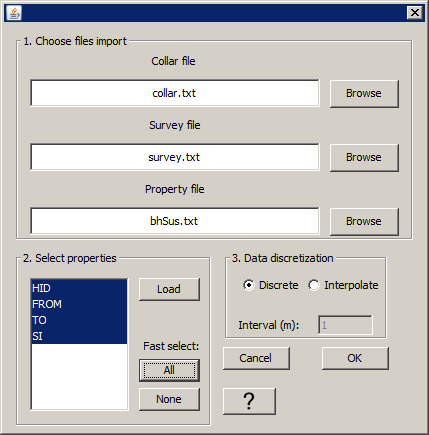
\includegraphics[width=0.8\textwidth]{images/BHSS/BHimport1.PNG}}
    \caption{The first \ac{GUI} for importing bore hole data}
    \label{fig:BHimport1}
\end{figure}

There are two methods to link property and drilling data,  ``Discrete'' and ``Interpolate''. If the ``Discrete'' option is selected then GIFtools simply determined the spatial location based on the depth provided in the property file. In the case that the depth is given in the form of intervals, the depth of the measurement is considered to be the midpoint of the interval. 

If ``Interpolate'' is selected the program behaves differently depending on whether the depth information is simple depths or intervals. In both cases instead of using the depth information directly, a sample is provided at each point along the bore hole with distances between each sample defined by the sampling interval value in the first \ac{GUI} (\autoref{fig:BHimport1}).

In the case of simple depths, it is assumed that the measurement is some physical property, and given the sample depths the measurements are linearly interpolated along the bore hole. In the case of intervals it is assumed that the measurement lithologies should not be interpolated, so samples with depths that are within an interval are assigned the property given while depths outside of any range are assigned a NaN (not a number) value.

Once the files, and property location options have been set, the next step to importing bore hole data into GIFtools is the set of data columns and data headers. Since different collar, survey, and property files have different column orders it advantageous to allow the flexibility to assign columns with a given header to any property of the bore hole object in GIFtools. The \ac{GUI} to assign the columns is shown in \autoref{fig:BHimport2}

 \begin{figure} [h]
    \centering
    \frame{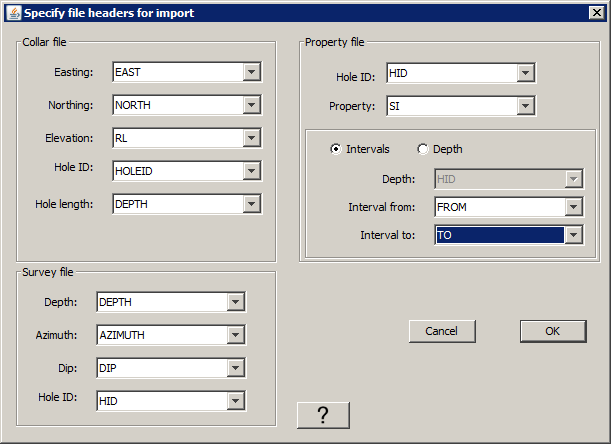
\includegraphics[width=0.8\textwidth]{images/BHSS/BHimport2.PNG}}
    \caption{The file header \ac{GUI} for importing bore hole data}
    \label{fig:BHimport2}
\end{figure}

\subsection{Visualizing Bore Hole Data}
\label{subsec:visBH}

As stated in the introduction to this section, one of the advantages of integrating the Model Builder tools (including these tools for bore hole data being described) into GIFtools, a more general data visualization and quality control environment, is the ability to use those same tools for the data with which we create regularizations. In this case it is very useful to be able to visualize bore hole data before it gets incorporated in reference model and bounds of an inversion. 

\autoref{fig:TKCBHvis} shows the visualization of the bore hole data from TKC. Note that the data has been sampled within each unit.  \autoref{fig:EPBHvis} shows the visualization of a physical property bore hole data set from El Poma. Note that instead of the method used in \autoref{fig:EPBHvis}, each datum along the hole was given its own position, in this case, the mid point of each small interval provided. In both cases the value of the visualized property of a given hole is shown along the side of the 3D representation of all the holes.

 \begin{figure} [h]
    \centering
    \frame{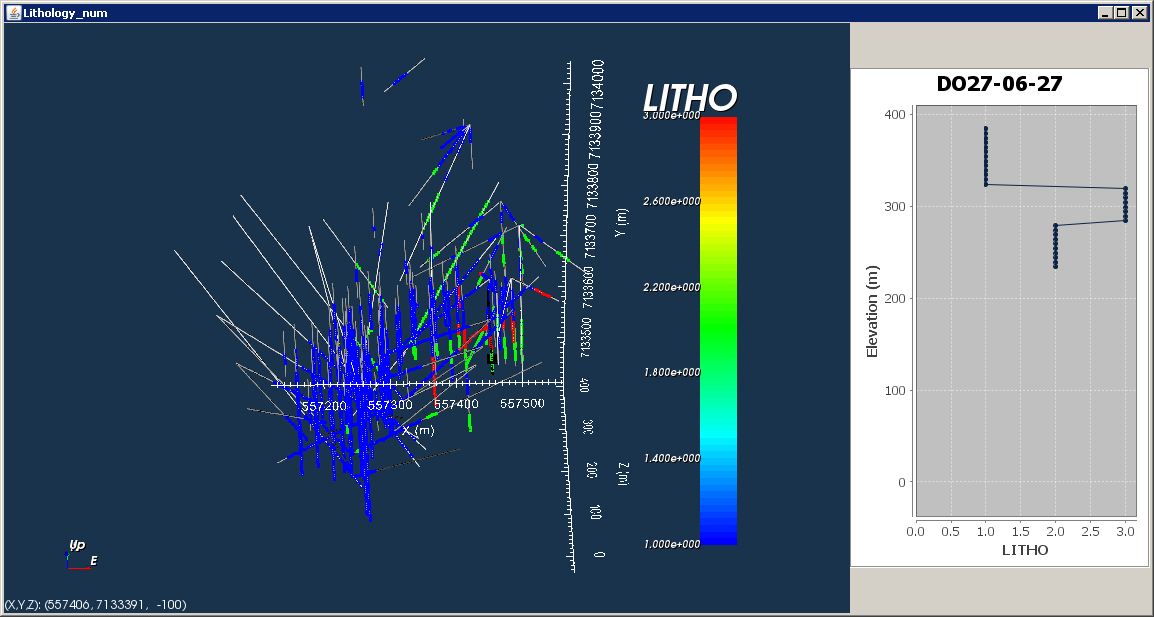
\includegraphics[width=0.8\textwidth]{images/BHSS/TKCBHvis.PNG}}
    \caption{Visualization of TKC lithology bore hole data}
    \label{fig:TKCBHvis}
\end{figure}

 \begin{figure} [h]
    \centering
    \frame{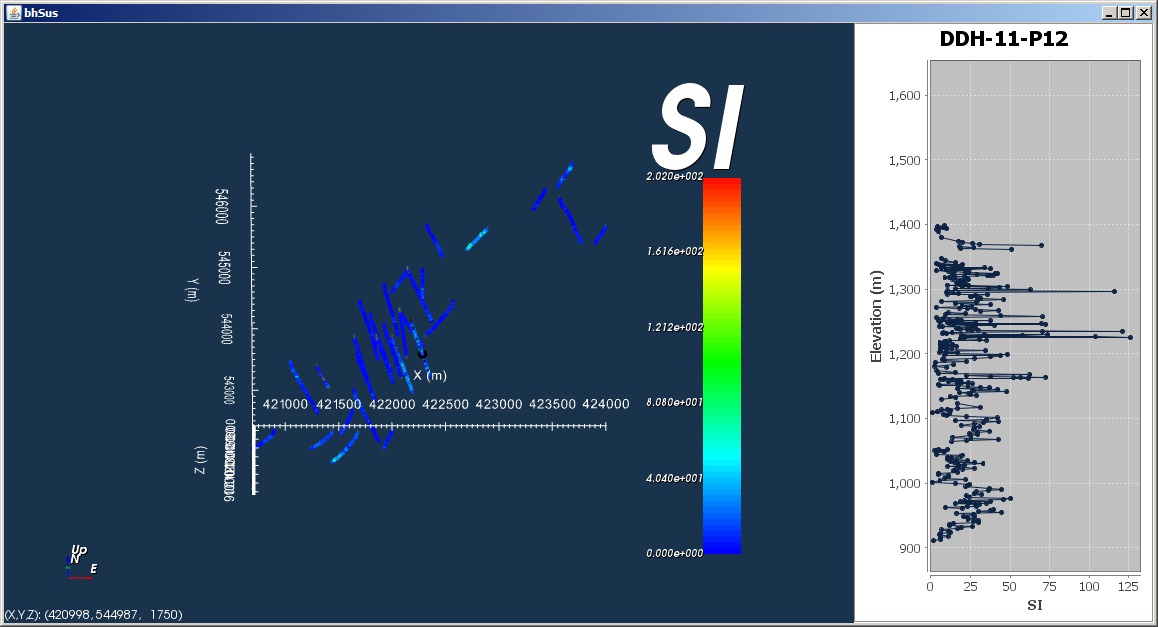
\includegraphics[width=0.8\textwidth]{images/BHSS/EPBHvis.PNG}}
    \caption{Visualization of El Poma susceptibility bore hole data}
    \label{fig:EPBHvis}
\end{figure}

\subsection{Discretizing Bore Hole Data}
\label{subsec:discBH}

Before a bore hole data set can be use in the creation of inversion constraints, it needs to be discretized on the mesh that will be used in the inversion. Discretization allows the multiple data along each bore hole to be usable in the context of an inversion on a given mesh. This will allow the creation of reference models, bounds, and weights. 

The process to discretized bore hole data in GIFtools and Model Builder is as follows.

\begin{itemize}
 \item Provide mesh. If the bore data will be used with a Model Builder module to create constraints, it must have the same mesh as the Model Builder module.
 \item describe distribution 
 \begin{itemize}
  \item normal
  \item log normal
%   \item describe why one and not other. Cond tends to be log normal (citation needed), Den tends to be normal (citation needed), Susc can be either depending on who you ask(citation needed).
 \end{itemize}
 \item describe method of determining bounds
 \begin{itemize}
  \item Confidence interval: given a number of samples in a cell and a distribution, bounds are determined from a given percent confidence interval. Where the standard deviation is zero, (if there is only one datum, or all the data are equal) he minimum value is used in place of the confidence interval.
  \item Floor: Simply assigns a bound based on the mean value of each cell plus or minus the provided floor value
  \item Standard Deviation: Calculates the standard deviation of the sample values in each mesh cell (given a normal or log normal distribution). The bounds are set as equal to the mean value plus some multiple of the standard deviation. In the case that the standard deviation is zero the minimum value is used instead of the multiplied standard deviation. 
 \end{itemize}
 \item positivity simply set the lower bound and mean to be at least 0
\end{itemize}

 \begin{figure} [h]
    \centering
    \frame{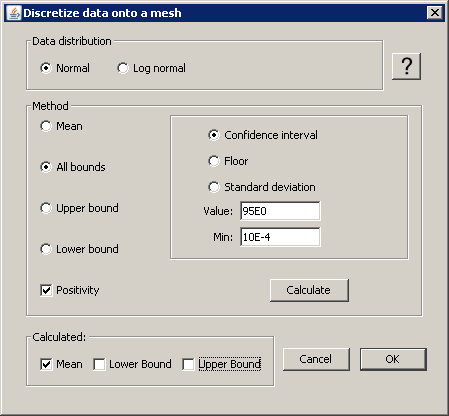
\includegraphics[width=0.8\textwidth]{images/BHSS/disc.PNG}}
    \caption{\ac{GUI} to allow the discretization of bore hole data to a given mesh}
    \label{fig:disc}
\end{figure}

\autoref{fig:disc} shows the GIFtools \ac{GUI} that allows the user to input the discretization options.

\subsection{Linking Lithology Information into Petrophysical Information}
\label{subsec:lithBH}

As stated in the introduction of this section, bore hole data often consists of lithology data instead of a physical property. In these cases the lithology information needs to be converted into petrophysical information so that the bore holes are to be used to constrain inversion results. In GIFtools, linking lithology information to petrophysical data is done by what is called a geology definition. The geology definition is a lookup table that contains information of each particular geological unit's property, lower and upper bounds, and optionally the smallness weight associated with each unit. 

Using the geology definition we can convert a geology model that has information about the spatial distribution of geological units but not of their physical properties into constraints that are usable by an inversion. \autoref{fig:geoDefBH} is an example of a geology definition in the GIFtools GUI. The data in the geological definition came from lab measurements of magnetic susceptibility and remancence within each geological unit.

 \begin{figure} [h]
    \centering
    \frame{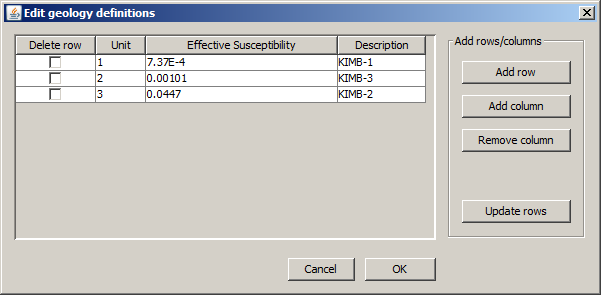
\includegraphics[width=0.8\textwidth]{images/BHSS/geoDefBH.PNG}}
    \caption{The geology definition of the lithological units in the TKC bore hole data. Effective susceptibility is measured in SI is (in this case)}
    \label{fig:geoDefBH}
\end{figure}

Once the geology definition is set the lithological bore hole can be treated as a physical property bore hole data set where each sample of a given unit is assigned the property in the geology definition. Multiple properties can be stored in the geology definition and the one that will be used to create a set of constraints can be changed by editing the geology definition's I/O header.

\subsection{Editing Bore Hole Data}
\label{subsec:visBH}

\begin{itemize}
 \item show editing of BH discretization
 \item show editing of prop data for susc to eff susc
\end{itemize}

\subsection{Making Constraint}
\label{subsec:makeConstBH}

\begin{itemize}
 \item show resolve conflicts dialogue
 \begin{itemize}
  \item steal from below section (new images necessary)
 \end{itemize}
\end{itemize}

\subsection{Including Surface Sample Information in Inversion Regularization}
\label{subsec:SS}

In addition to physical property measurements down hole, physical properties can also be measured on the surface, in many cases with much more ease. As with bore hole data, much work  has been done on including surface sample information in inversion regularization. Surface samples take on increased importance since in forward models the sensitivity of the data on a given cell is higher when the cell is nearer the surface. Constraining these surface cells can reduce artifacts that come from this increased sensitivity.

\begin{itemize}
 \item importing SS
 \item visualize
 \item editing 
 \item creation of constraints
\end{itemize}

\section{Including Geological Maps in Inversion Regularization}
\label{sec:maps}

It is often the case that geological information is provided in the form of geological maps in either cross section or plan view. Such maps are particularly useful since they provide a great deal of information over their entire surface. Cross sections can provide information at depth and constrain a whole region often within the center of a target of interest. Plan view maps do not provide information at depth, but they do constrain the entire surface of the region being inverted.  Constraining the surface of an inversion is of interest since the sensitivity of the data to the top cells is particularly high, which can lead to artifacts on the surface. For the next section the plan view model is from the El Poma case study and the cross section model is from TKC, specifically the map from \citep{harder2006geology}

\cite{williams2008geologically} discuses methods to include maps in the form of ESRI shapefiles. His method has the disadvantage of not being able to incorporate information from maps stored a pixel images. On the other hand, a method that allows the incorporation of pixel images allows the use of ESRI shapefiles since the conversion of a shapefile to a pixel image is trivial.

Below is the method I have developed to incorporate pixel maps.

\subsection{ Preprocessing images}
\label{subsec:Preprocessing images}

Often a geological map image will not be immediately suitable to the methods used below and some prepossessing is required. The most notable features that are undesirable in a map are geological units that are not only one or two colours and text or other annotations that could be interpreted by the program as geological information. Also map images may be of too high resolution to be efficiently used in these methods and must also be down-sampled to save  computer processing time and memory.

 \begin{figure} [h]
    \centering
    \frame{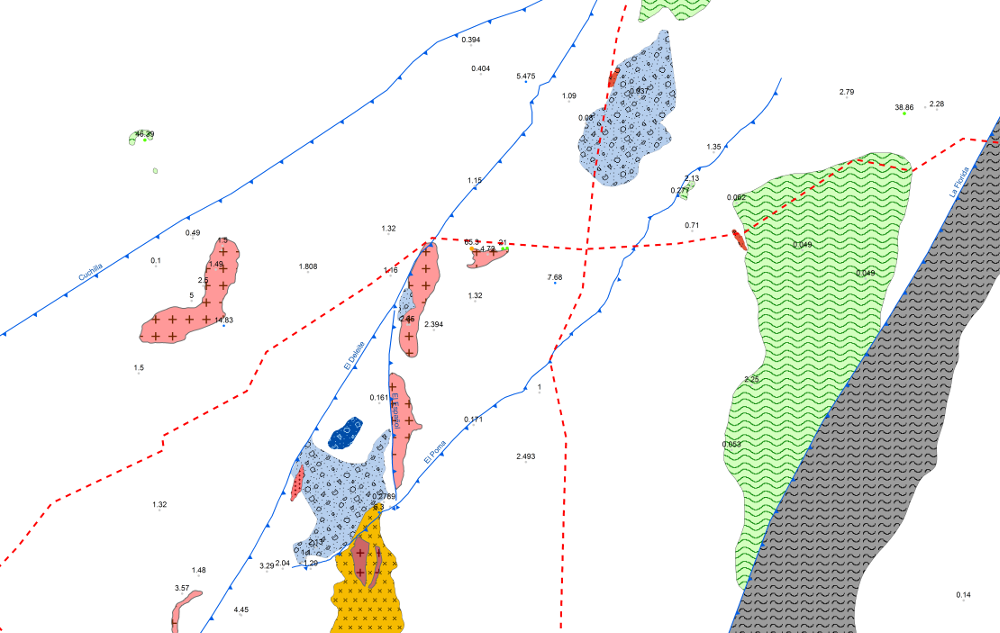
\includegraphics[width=0.8\textwidth]{images/Faults/ElPoma_GEOL_MagSus.png}}
    \caption{The El Poma map with fault lines (blue lines with barbs) included}
    \label{fig:ElPoma_GEOL_MagSus}
\end{figure}

For example \autoref{fig:ElPoma_GEOL_MagSus} has great deal of information, (faults, magnetic susceptibility surface samples, etc.) that are not information about geological units. In addition the geological units are not a single colour polygon. The image has been edited in the GNU Image Manipulation Program (GIMP), a free image editing program, to produce \autoref{fig:ElPoma_GEOL_MagSus_M2M_downsample8}. 

 \begin{figure} [h]
    \centering
    \frame{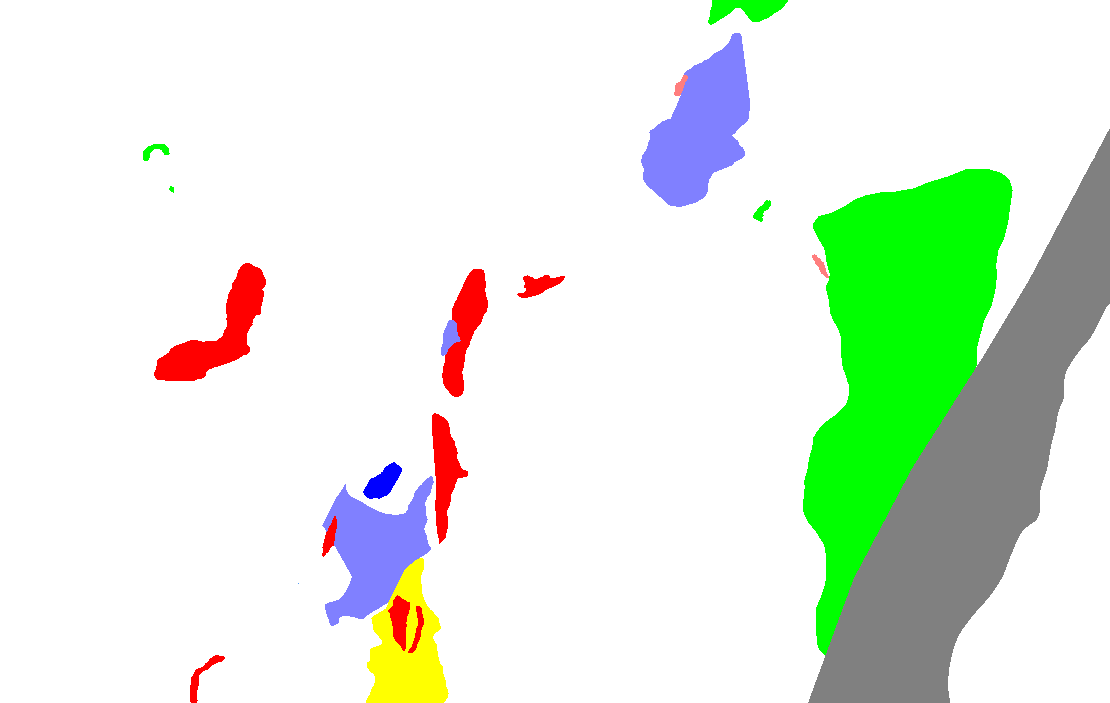
\includegraphics[width=0.8\textwidth]{images/MaptoModel/ElPoma_GEOL_MagSus_M2M_downsample8.png}}
    \caption{The El Poma map with extra information removed and geological units made a single colour}
    \label{fig:ElPoma_GEOL_MagSus_M2M_downsample8}
\end{figure}

\FloatBarrier
\subsection{Loading Images into GIFtools}
\label{subsec:Load Images into GIFtools}

\begin{itemize}
\item load image into the GIFtools format (\autoref{fig:importPlanGui})
\begin{itemize}
	\item Determine image format.
	\item Load image using MATLAB utilities.
	\item Convert image into .png style representation for faster computation.
	\item Using .twf file (world file) assign location and spacial resolution to the image.
	\item Assign a legend linking pixel RGB values to geological unit.
	\item Assign topography (either number or GIFtools TOPOdata item) for visualization.
	\begin{itemize}
		\item In the case of a cross section image, instead of topography, information for the location of the cross section in 3D or 2D space is required (\autoref{fig:importCrossGui}).
	\end{itemize}
\end{itemize}
\end{itemize}
\begin{figure} [h]
    \centering
    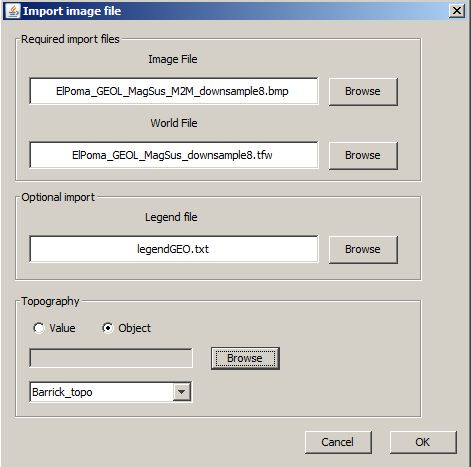
\includegraphics[width=0.5\textwidth]{images/MaptoModel/importPlan.PNG}
    \caption{\ac{GUI} for importing plan view image }
    \label{fig:importPlanGui}
\end{figure}
\begin{figure} [h]
    \centering
    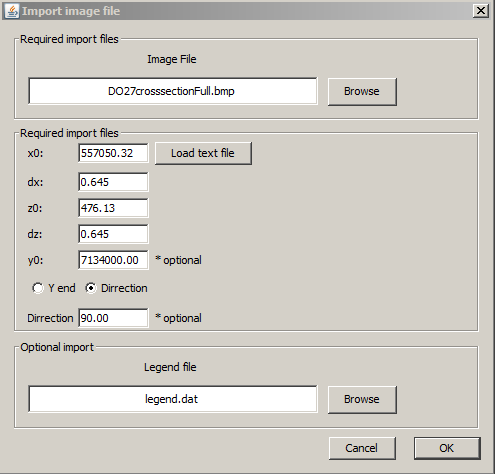
\includegraphics[width=0.5\textwidth]{images/MaptoModel/importCross.PNG}
    \caption{\ac{GUI} for importing cross section image }
    \label{fig:importCrossGui}
\end{figure}
Storing a map as a GIFtools object allows its use in several ways. Notably it allows the integration of the map with models and data, allowing figures overlaying the map and data or model and allowing interpretation of the data or model with direct reference to the map (\autoref{fig:mapData}).
\begin{figure} [h]
    \centering
    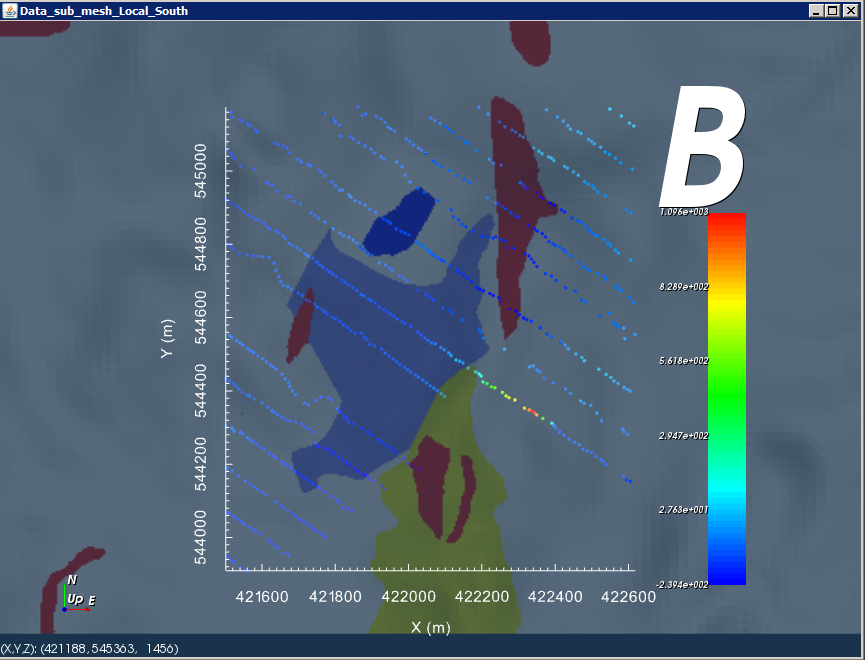
\includegraphics[width=0.5\textwidth]{images/MaptoModel/mapData.PNG}
    \caption{Example of magnetics data being viewed with a map overlaid }
    \label{fig:mapData}
\end{figure}



\subsection{Creating a Pixel Map Legend}
\label{subsec:Create Pixel Map Legend}

Continuing on in the process of making a geological constraint.
\begin{itemize}
\item Find the geological unit represented of each pixel.
\begin{itemize}
	\item In the .png style format as stored in MATLAB, an image consists of an ``image'' field, a matrix of integers, and a ``map'' field, which maps the image matrix to RBG value triplets.
	\item Each RGB triplet is compared to the legend that was provided when the image was loaded. A map field entry is considered to represent a geological unit if all three components of the RGB triplet are within a provided tolerance of any entry in the legend.
	\item Now that we have a relation of entries in the map field to geological units in the legend, we can assign a geological unit to each pixel in the original image simply by applying the new geological map to the image field.
\end{itemize}
\end{itemize}

\subsection{Making a Geology Model from Map}
\label{subsec:Make Geology Model from Map}

\subsubsection{Plan View}
\label{subsubsec:Make Geology Model from Map Plan View}

\begin{itemize}
\item Provide active model. For convenience this is usually an active model already associated with a Model Builder object.
\begin{itemize}
	\item The active model simultaneously provides a discretized topography for the map to lay along and also a mesh (\ac{GIF} 3D tensor or OcTree).
\end{itemize}
\item Provide some form of depth information.
\begin{itemize}
	\item Thickness, a certain amount of depth below topography at each point will be assigned the geological unit at each.
	\item Depth, the map will be used to assign a geological unit down to a fixed depth across the whole model.
	\item Surface, if you provide another surface below topography the cells between topography and the other surface will be assigned.
\end{itemize}

\item Crop all pixels that extend outside of the mesh or that represent the background geological unit.
\begin{itemize}
	\item The cropping greatly speeds up the process and makes it require much less computer memory.
	\item Furthermore, in the event of a mistake with coordinates the process ends almost instantly as there are few pixels to process.
\end{itemize}
\item Finally the geological model is created.
\begin{itemize}
	\item We determine which cell of the mesh each pixel is in, including those cells below each pixel to account for thickness.
	\item Each cell is assigned a geological unit based on the mode of the geological values of each pixel which colours that cell.  In other words, each cell is identified with the geological unit which fills the greatest proportion of the cell.
	\begin{itemize}
	\item The mode is used since each cell will be a particular unit. Since the property being mapped onto each cell by construction must represent a single geological unit, interpolation between the units will not provide the desired result.
	\end{itemize}
	\item The geology definition which will allow the assignment of physical properties to each geological unit. The result is shown in \autoref{fig:mapModelPlan}, the continuous colour bar is not an indication of a continuous model. All model values are integers that represent geological units in the map.
\end{itemize}
\end{itemize}
\begin{figure} [h]
    \centering
    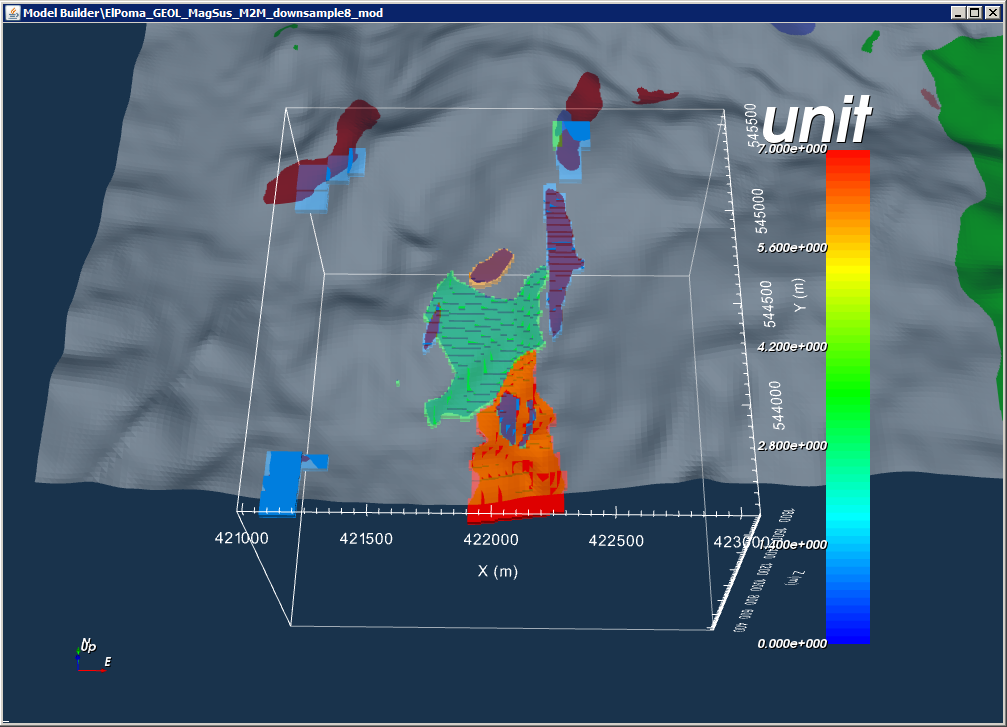
\includegraphics[width=0.5\textwidth]{images/MaptoModel/mapModelPlan.PNG}
    \caption{Example of a geology model created from a map with the map overlaid}
    \label{fig:mapModelPlan}
\end{figure}

\subsubsection{Cross Section}
\label{subsubsec:Make Geology Model from Map Cross Section}

The cross section case follows much the same procedure with a few exceptions. An imported cross section map is shown overlaid on a 2D mesh in \autoref{fig:mapMeshCross}. Notably no parameter for the vertical extent is needed. The other notable exception is that mesh that is used is a \ac{GIF} 2D mesh. The result is shown in \autoref{fig:mapModelCross}.  

A 2D Geology model can be used to create constraints for a 2D inversion, it can also be used to add constraints to a 3D inversion as well. After the 2D geology model is created from the cross section map, it can be inserted into a 3D mesh (\ac{GIF} 3D tensor or OcTree) given a starting and ending position or a starting position and a direction \autoref{fig:add2Dto3D},\autoref{fig:mapModelCross3D}.

\begin{figure} [h]
    \centering
    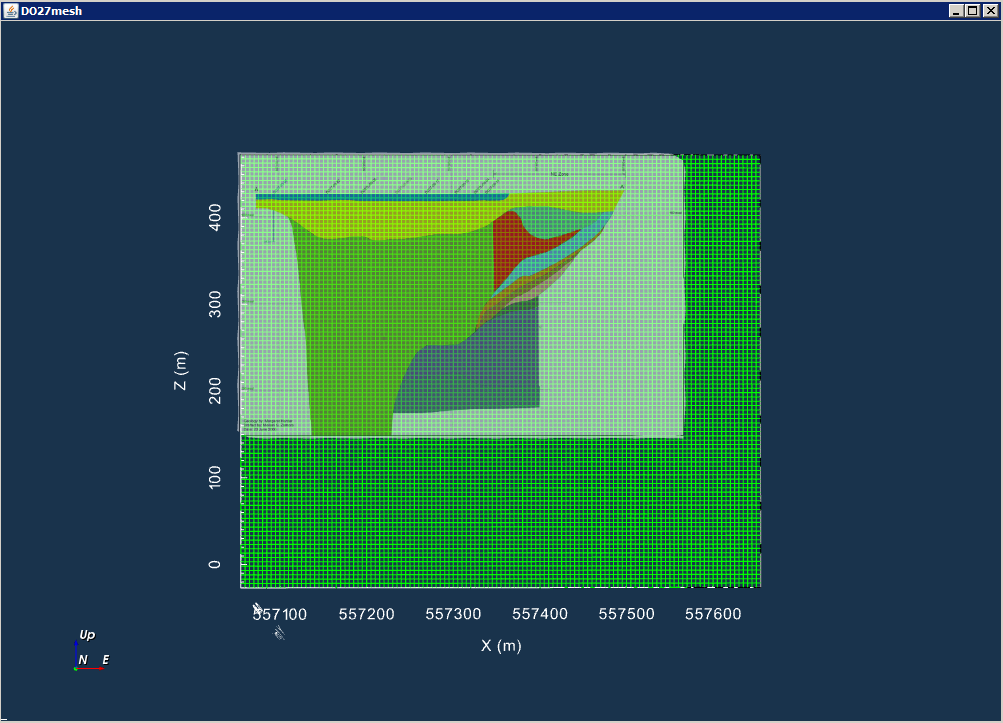
\includegraphics[width=0.5\textwidth]{images/MaptoModel/mapMeshCross.PNG}
    \caption{Example of a 2D mesh with the map overlaid}
    \label{fig:mapMeshCross}
\end{figure}
\begin{figure} [h]
    \centering
    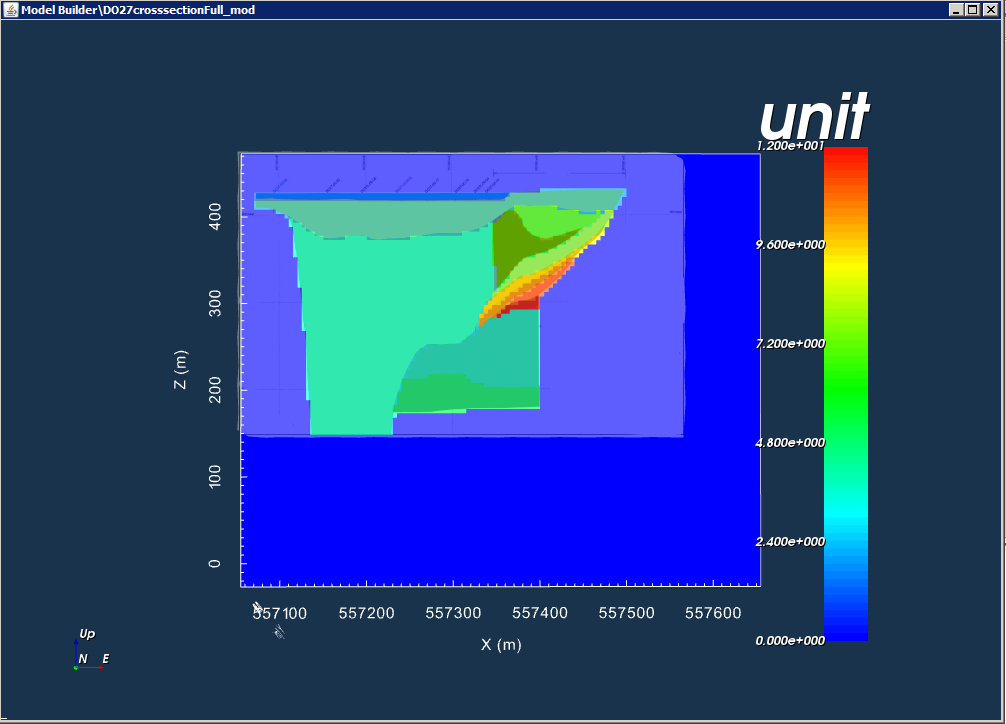
\includegraphics[width=0.5\textwidth]{images/MaptoModel/mapModelCross.PNG}
    \caption{Example of a 2D geology model created from a cross section map with the map overlaid}
    \label{fig:mapModelCross}
\end{figure}
\begin{figure} [h]
    \centering
    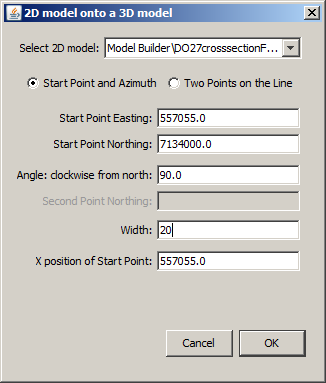
\includegraphics[width=0.5\textwidth]{images/MaptoModel/add2Dto3D.PNG}
    \caption{GUI for adding a 2D model to a 3D model}
    \label{fig:add2Dto3D}
\end{figure}
\begin{figure} [h]
    \centering
    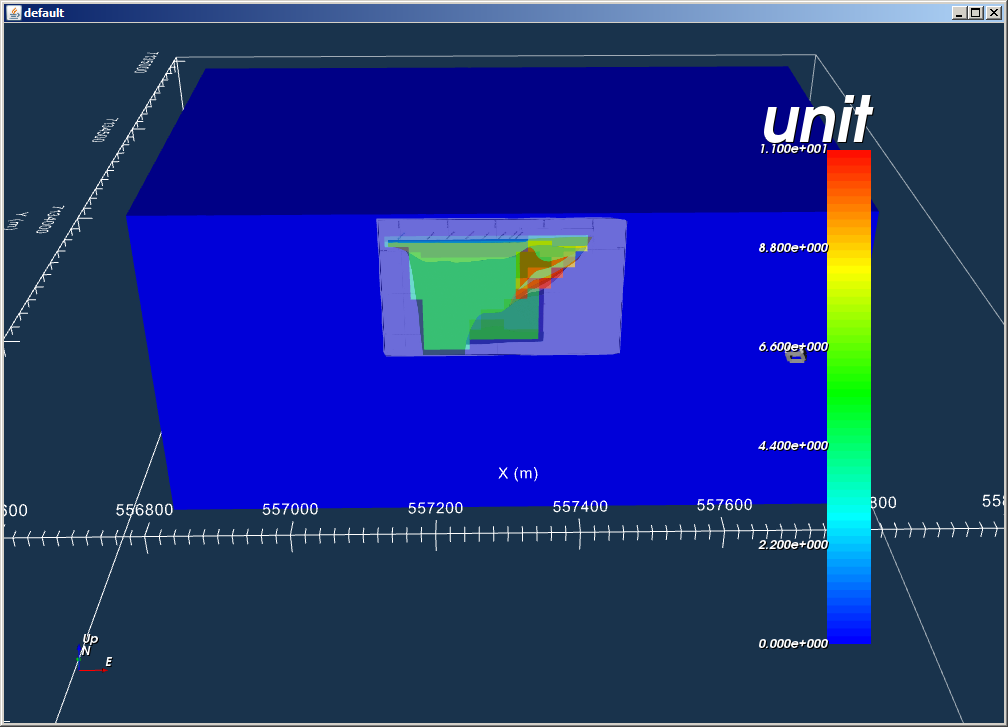
\includegraphics[width=0.5\textwidth]{images/MaptoModel/mapModelCross3D.PNG}
    \caption{Example of a 2D geology inserted into a 3D model with the map overlaid}
    \label{fig:mapModelCross3D}
\end{figure}
\FloatBarrier
\subsection{Making Constraints for an Inversion}
\label{subsec:Making Constraints for an Inversion}

The model that has been created is a geology model. That is, a model in which each cell represents a given geological unit. To be able to convert this model into a constraint for a geophysical inversion the link between between the geology and the petrophysics needs to be provided. 

The link is stored in what is called a geology definition. In GIFtools this takes the form of a lookup table that contains information of each particular geological unit's property, lower and upper bounds, and optionally the smallness weight associated with each unit. 

Using the geology definition we can convert a geology model that has information about the spatial distribution of geological units but not of their physical properties into constraints that are usable by an inversion. In the figures below the geological definition came from surface measurements of magnetic susceptibility within each geological unit. \autoref{fig:geoDefPlan} is an example of a geology definition in the GIFtools GUI.
\begin{figure} [h]
    \centering
    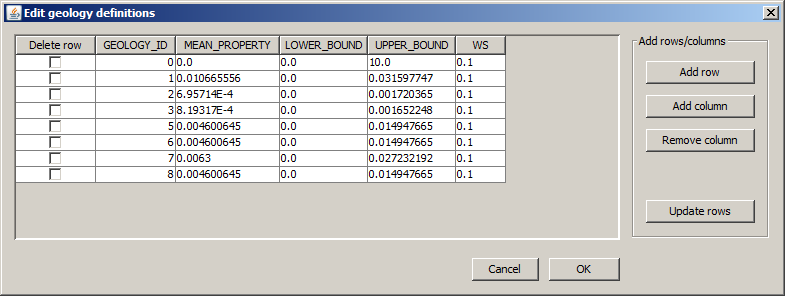
\includegraphics[width=0.8\textwidth]{images/MaptoModel/geoDefPlan.PNG}
    \caption{Example of a geological definition as displayed in the GIFtools GUI, the Mean Property, and Bounds are susceptibility measurement in SI$\times10^-3$ and the WS is to set the smallness weight model.}
    \label{fig:geoDefPlan}
\end{figure}

Once the geology definition is provided, we can use the Combine Model Dialog (\autoref{fig:combineModelRef}) in Model Builder to create a reference model and bounds. 
\begin{figure} [h]
    \centering
    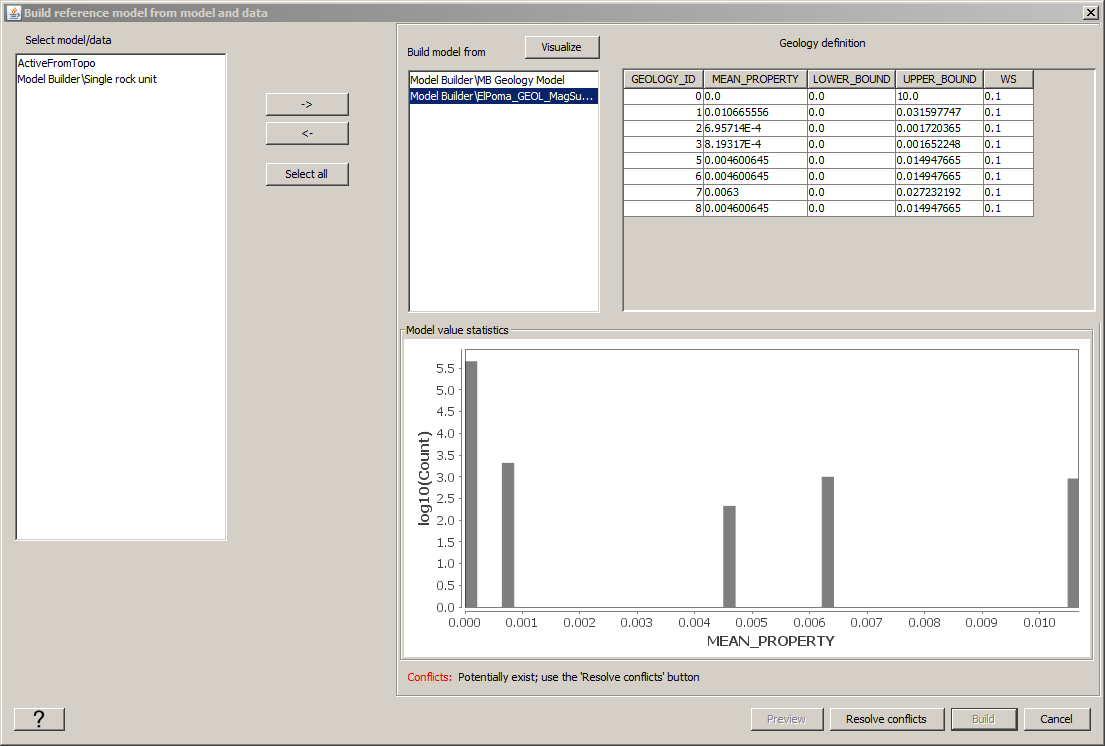
\includegraphics[width=0.8\textwidth]{images/MaptoModel/combineModelRef.PNG}
    \caption{Example of a typical combine model dialog for a reference model}
    \label{fig:combineModelRef}
\end{figure}
In this case the resolution of conflicts is trivial as there is a single source of information. Less trivial examples of the creation of reference models and bounds will be discussed later. The resulting reference model is shown in \autoref{fig:mapRefModPlan}.
\begin{figure} [h]
    \centering
    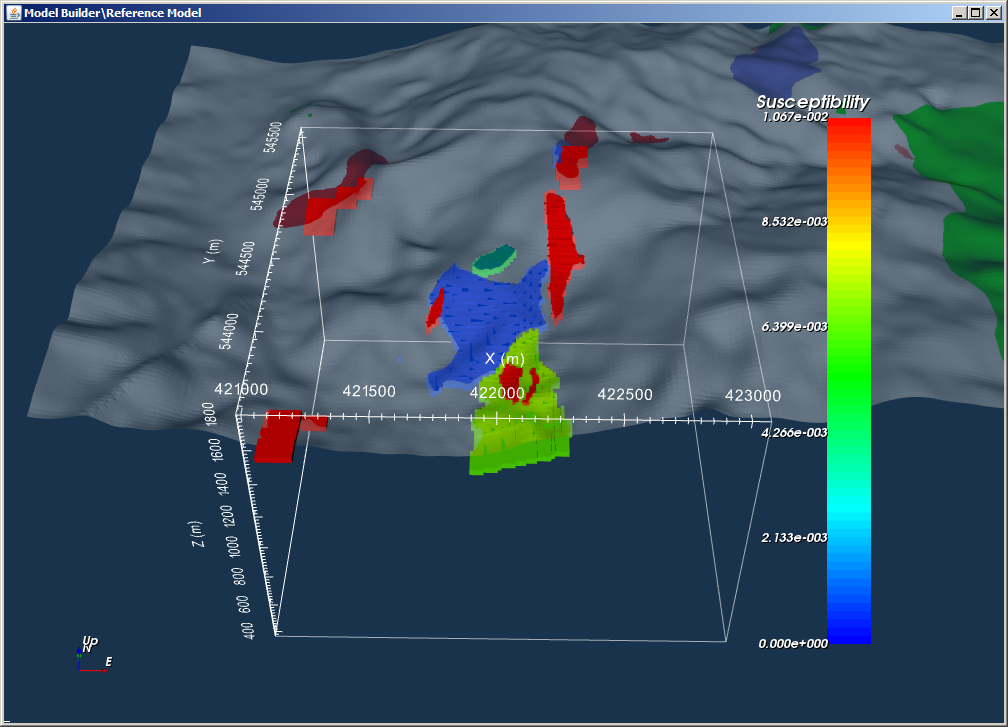
\includegraphics[width=0.8\textwidth]{images/MaptoModel/mapRefModPlan.PNG}
    \caption{Example of a reference model created from a geological map}
    \label{fig:mapRefModPlan}
\end{figure}

\subsection{Inputing Fault information from Geological Maps}
\label{subsec:Inputing Fault information from Geological Maps}

Another piece of information that can be in geological maps are fault locations. Again in the context of El Poma the map provided a whole complex of thrust faults as shown in the un-doctored map in \autoref{fig:ElPoma_GEOL_MagSus}

The method used to insert faults into an inversion is as follows:

\begin{itemize}
\item Determine the end points of the fault.
\begin{itemize}
	\item GIFtools makes this easy by reporting the location of the cursor in the data viewer allowing you to find the location (including elevation) of a point along the fault.
\end{itemize}
\item Using the locations provided GIFtools creates the fault weights by creating a two boxes, each with one of its sides along the fault location as defined in the \ac{GUI}. By setting the value of cells in each box to one, and then taking the derivative of each of models that had a box added, two face models are created. The location of faces along the fault can be determined by taking the non-zero faces that are in common between the two models.  It is then possible to set the values of the the faces that define the fault to any value desired.

\item faces within this box are assigned a new value that is provided in the GUI \autoref{fig:makeFaultGUI}.
\end{itemize}

\begin{figure} [h]
    \centering
    \frame{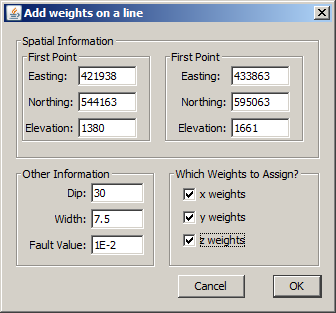
\includegraphics[width=0.5\textwidth]{images/Faults/makeFaultGUI.PNG}}
    \caption{The GUI for the creation of fault weights}
    \label{fig:makeFaultGUI}
\end{figure}

This process can be done multiple times along several consecutive segments of multiple faults to create fault complexes that are not straight of have multiple faults, as shown in \autoref{fig:faults}

\begin{figure} [h]
    \centering
    \frame{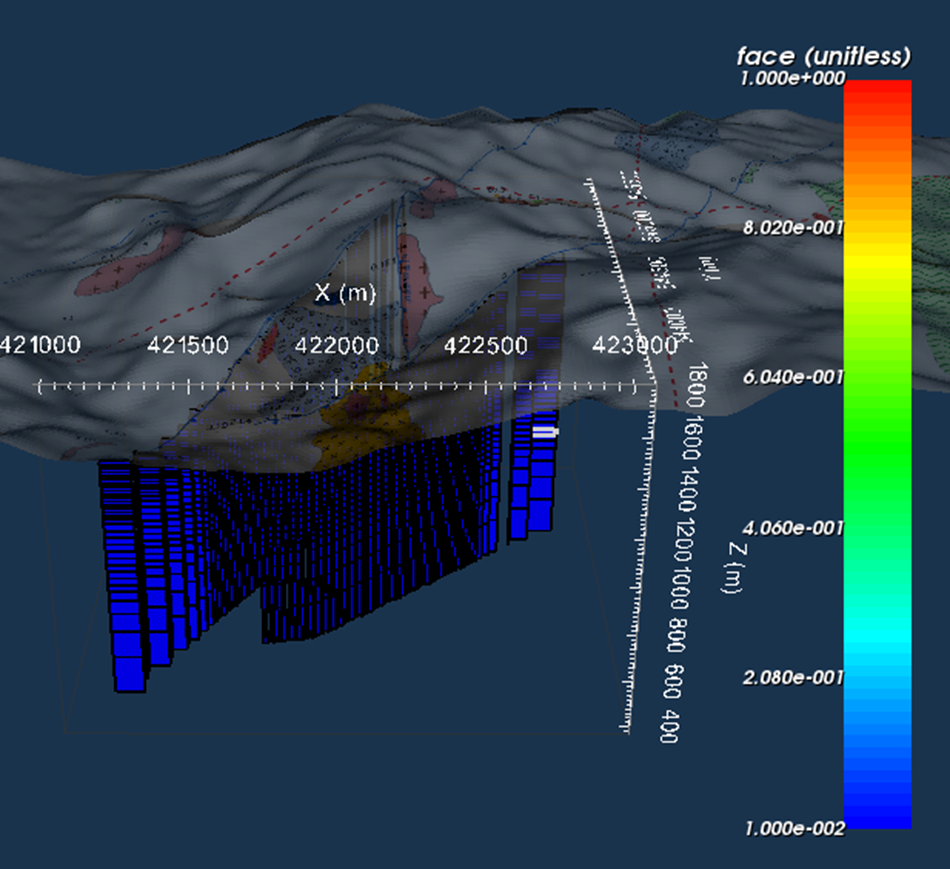
\includegraphics[width=0.5\textwidth]{images/Faults/faults.png}}
    \caption{An example of fault weights that can be created with GIFtools. In this case a vertical fault (no dip) was created and the blue curtain is the low face weights that define the fault in an inversion. Only the faces that have values that are not 1 are visualized. Since the faces are set at a lower value than the rest of the face model (1) they are shown as blue.}
    \label{fig:faults}
\end{figure}
\FloatBarrier

\section{Clustering to Create Constraints}
\label{sec:cluster}

\subsection{Clustering Algorithms}
\label{subsec:clusterAlgo}

In contexts where multiple data types have been collected over an area, it is often of interest to include information from one inversion result (from one data type) in the regularization of another (likely of a different data type). Much work has been done on this topic (see \autoref{subsec:litrevLitho}). 

One possible way of integrating information into one inversion from another inversion result is through clustering the recovered models to create pseudo-geological models, and then using these to create reference models, bounds, and smoothness weights to constrain subsequent inversions. By pseudo-geologic I mean a geologic type model that has discrete units and a geologic definition that links them to physical propoerties, but which is not the result of a geological interpretation of surface or depth litholgical data. Rather pseudo-geological models in this thesis tend to be the result of clustering multiple inversion results.

Given several inversions of different data types, multiple models of different physical properties can be recovered. Assuming that each recovered model is on the same mesh (either because all inversions were performed on the same mesh or they were interpolated onto the same mesh after the fact) each cell has a value for each physical property. Since the standard representation of a model is a vector $\mathbf m \in \mathbb R^M$ where as in \autoref{eq:forwardProb} $M$ is the number of cells in the discretization of the earth model, we can generalize so that $\mathbf M \in \mathbb R^{M\times l}$ is the compiled results of $l$ inversions. This notation allows us to say that $\mathbf M$ is made out of several $m_i$ for $i = 1 \cdots M$ and where each $m_i$ is a row vector $l$ long.

In each case the algorithm depends on the user providing the number of clusters for analysis. The clustering method used determines the clusters and the membership of each $m_i$ in the clusters.

The first clustering methods implemented in Model Builder is simply a set of user defined boundaries. These allow a great deal of user control and can be very useful assuming something is known about the underground geology or the physical properties of given units. On the other hand, it can quickly be untenable to use this method if several clusters are needed or many recovered models are being clustered.

The second clustering method implemented in Model Builder is k-means clustering \cite{gaf1984multivariate} which is based on the minimization of the following objective function,

\begin{equation}
 \phi_{k\text{-}mean} = \sum_{j=1}^k\sum_{m_i \in S_j}\|m_i - v_j\|_2^2, \label{eq:kmean}
\end{equation}


where $k$ is the number of clusters and $S_j$ are the sets of model cells $m_i$ that make up the clustering, finally $v_j$ are the centroids of each cluster, that is the central tendency of the data included in the given cluster $S_i$. The algorithm to minimize $\phi_{\text{k-mean}}$ is a two step process firstly assigning each $m_i$ to a cluster $S_j$ and secondly determining a new set of $v_j$ that better fit the data.

Finally, the third clustering algorithm implemented in Model Builder is \acf{FCM} \citep{sun2015multidomain}. \ac{FCM} is a generalization of \autoref{eq:kmean} where instead of each datum $m_i$ being in only one cluster, each datum is assigned membership in each cluster to varying degrees allowing ``fuzziness'' in the classification. The objective function becomes

\begin{equation}
 \phi_{FCM} = \sum_{j=1}^k\sum_{i = 1}^Mu^q_{ij}\|m_i - v_j\|_2^2,\label{eq:fcm}
\end{equation}

where instead of the $k$ sets $S_j$, membership in each cluster is represented by the membership matrix $u \in \mathbb R^{M\times k}$. Each row of $u$ must sum to 1, in other words each datum is is evenly weighted in the algorithm but may be classified as partially in each cluster. Finally $q$, controls the ``fuzziness'' of the clustering with a value of $q = 1$ making a non-fuzzy clustering with each datum being in only one cluster and amount that a given datum can be in multiple clusters increasing as the value of $q$ increases. A standard value of $q$ is 2.

In the case of the clustering algorithm used in Model Builder the final step is ``de-fuzzification'', that is the determining of the cluster that each model cell most fits in. Each model cell is assigned the cluster for which it has the highest membership value.

In both the k-means and the \ac{FCM} case the minimization of the objective functions is done by the standard MATLAB function and notably the value of $q$ in the \ac{FCM} case is set at 2.

\subsection{Clustering In GIFtools and Model Builder}
\label{subsec:clusterTools}

\begin{itemize}
 \item describe requirements
 \item show GUI
 \item show result
\end{itemize}

\subsection{Creation of Constraints}
\label{subsec:clusterConstraints}

\begin{itemize}
 \item show creation of ref and bounds from mean cluster boundaries
 \item show creation of sharp bounds with weights.
\end{itemize}

\section{Voxel-Parametric Inversion to Provide Physical Property Values for Geological Models}
\label{sec:voxelParam}

In \autoref{sec:cluster} geological type models that span the whole discretized volume are defined. These are more extensive than the geological models described in \autoref{subsec:Make Geology Model from Map} because each cell is classified into a cluster as opposed to most cells not having any information (due to the map not intersecting the cell at all in the case of most cells).

In addition to pseudo-geological models created by clustering, it is also possible to get geological models from drill or surface geological data. In the TKC case study, one of the forms of geological data that was provided was a set of points created from the interpreted interfaces between units determined using the litholgical bore hole data shown in \autoref{fig:TKCBHvis}. The point cloud of the interfaces is shown in \autoref{fig:geoLoc} and the resultant geological model created using the ``add non-convex polyhedron'' command is shown in \autoref{fig:geoMod}.

\begin{figure} [h]
    \centering
    \frame{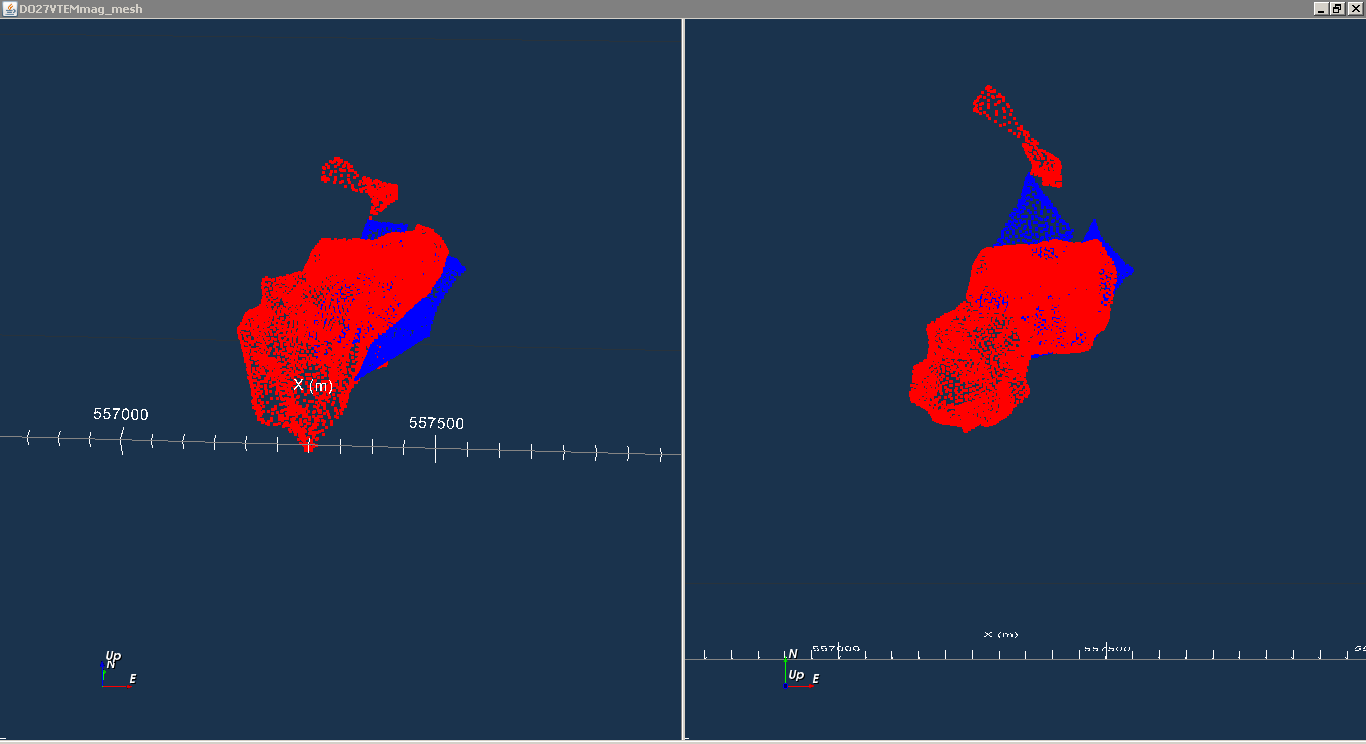
\includegraphics[width=0.5\textwidth]{images/BHSS/geoLoc.PNG}}
    \caption{Point cloud of the geological interfaces for TKC bore hole data}
    \label{fig:geoLoc}
\end{figure}

\begin{figure} [h]
    \centering
    \frame{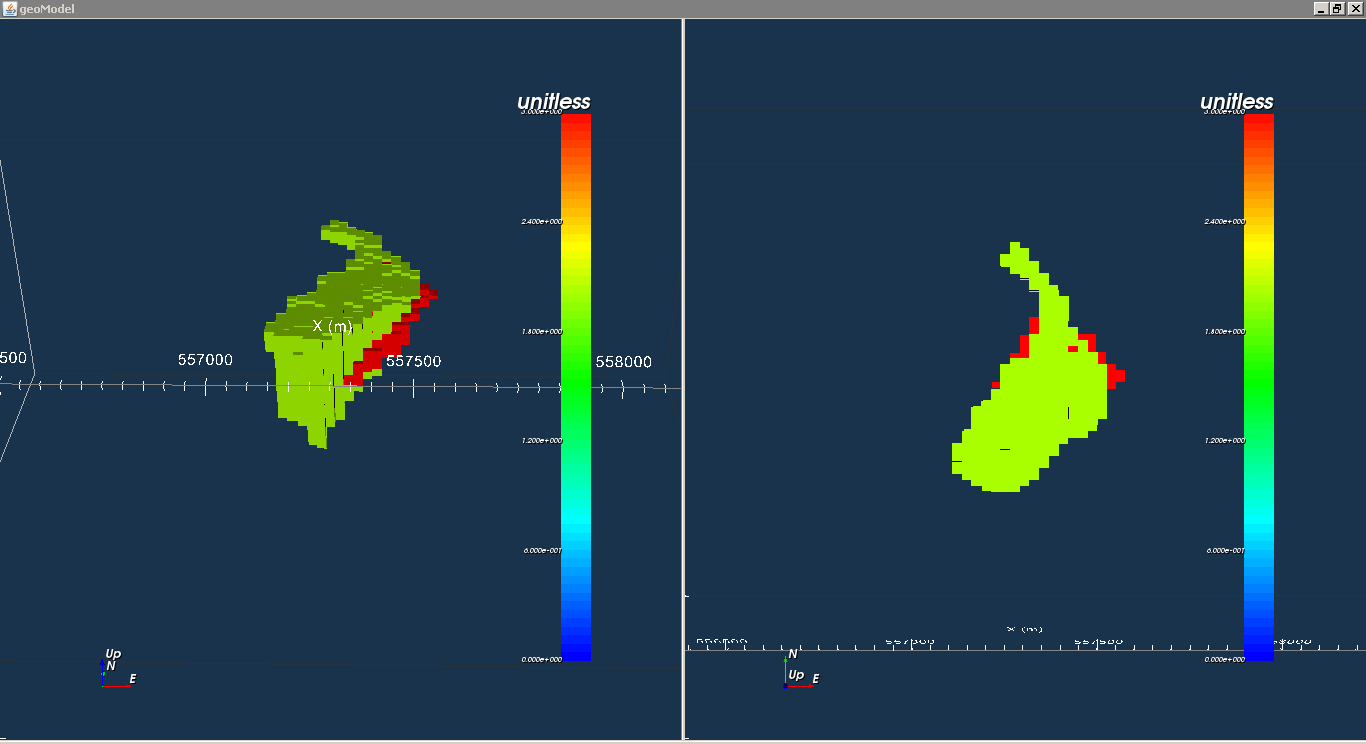
\includegraphics[width=0.5\textwidth]{images/BHSS/geoMod.PNG}}
    \caption{A geological model created from the data shown in \autoref{fig:geoLoc}}
    \label{fig:geoMod}
\end{figure}

In the cases listed in (the figure that shows a clustered model) and \autoref{fig:geoMod}, we have acquired a distribution of geological units that extend across the whole discretized volume it becomes interesting to go further into the assignment of physical properties to the geological units in question. For a clustered pseudo-geological model the obvious method of property assignment is simply using the centroid value recovered from the clustering algorithm. In addition a standard deviation from the mean can be acquired to set the upper and lower bounds of each unit.

Another option is the direct assignment of measured physical property values to the (pseudo-)geological units. This method has the advantage of directly incorporating physical property data into the inversion constraints. Direct assignment can be done through the GIFtools \ac{GUI} by editing the geologic definition of the geological model, and this method makes most sense when the model in question either is the products of geological modeling as in \autoref{fig:geoMod} or there is a strong parallel between the clustered units and actual geological units. 

In some cases the above method are not optimal. In the case of cluster centroids, artifacts in the inversion can lead to magnitudes in the recovered model not being quite in scale with the physical properties in the ground. Additionally this method only works if the geological model in question was derived through clustering. In the case of the direct assignment of measured physical properties to geological units, the properties often vary a great deal across the earth model. This can be due to large scale variation across the geological unit (such as by alteration) or small scale variation where, for example, one portion of a sample can be significantly more susceptible than another.

I have developed another method to assign physical properties to geological models which is well-described by the title ``Voxel-Parametric inversion''. It assumes that a given geological model has correctly determined the distribution of geological units and tries to fit a given geophysical data set assuming that each unit has a single physical property value that is constant across the unit. 

The method allows the assignment of physical properties to geological units based on the best fitting set of properties to a data set. This gives an advantage over the methods described above by avoiding some artifacts due to under-determined inversion and avoiding putting undue confidence in a small number of physical property measurements. The method also allows fast and efficient inversion of data without a large number of parameters since the forward problem is much less complex and regularization beyond the setting of the geological units is unneeded.

\subsection{Formulation of Voxel-Parametric inversion problem}
\label{subsec:voxelParamFormulation}

As stated in \autoref{sec:Regularized Inversion} and \autoref{eq:forwardProb}, the forward problem for which we are trying to find the inverse is formulated as follows
\begin{equation}
\mathbf d = \mathbb F [\mathbf m], \label{eq:forwardProbTools}
\end{equation}
where as stated above $\mathbf d \in \mathbb R^N$ is the geophysical data, $\mathbf m \in \mathbb R^M$ is the discretized model that describes the distribution of some physical property in the ground, and $\mathbb F$ is the forward operator that mediates between them. $\mathbb F$ can be considered to be a matrix of size $N\times M$ which in the case of a non-linear problem has a dependence on the model $\mathbf m$ but in the case of linear problem (such as potential field problems) there is no such dependence. \autoref{eq:forwardProbTools} can be re-written
\begin{equation}
\mathbf d = \mathbf F(\mathbf m)\mathbf m, \label{eq:forwardProbMat}
\end{equation}
where $\mathbf F \in \mathbb R^{N\times M}$, and in the case of a linear problem
\begin{equation}
\mathbf d = \mathbf F\mathbf m. \label{eq:forwardProbMatLin}
\end{equation}

In this formulation a geological model can be represented as a sparse matrix $\mathbf{M}_g \in \mathbb R^{M\times k}$ (where $k$ is the number of geological units) that marks the membership of each model cell in each cluster and a vector $\mathbf m_g \in \mathbb R^{k}$ that has the property of each unit. Using these definitions we can define the standard property model that is represented by a geological model as
\begin{equation}
\mathbf m = \mathbf M_g\mathbf m_g, \label{eq:geoMod}
\end{equation}
where $\mathbf m$ is a standard voxel model with the each value of each cell being the value assigned to geological unit of that cell. \autoref{eq:geoMod} can be inserted intro \autoref{eq:forwardProbMatLin} to form 
\begin{equation}
\mathbf d = \big(\mathbf F\mathbf M_g\big)\mathbf m_g, \label{eq:forwardProbMatLinGeo}
\end{equation}
where $\mathbf F\mathbf M_g \in \mathbb R^{N\times k}$ is created by a sparse matrix product and is significantly smaller than $\mathbf F \in \mathbb R^{N\times M}$.

Voxel-Parametric inversion now simply consists of minimizing the following data objective function modified from \autoref{eq:phid}
\begin{equation}
\phi_{d\text{-}geo} =\|\mathbf W_d\Big(\big(\mathbf F\mathbf M_g\big)\mathbf m_g - \mathbf d^{obs}\Big)\|^2
\end{equation}
\label{eq:phidGeo}
which is significantly less computationally expensive than a full voxel inversion since the forward problem is now much smaller, and no additional regularization is required since the problem is now over determined rather than under-determined.

\subsection{Uses of Voxel-Parametric inversion results}
\label{subsec:voxelParamUses}

 \begin{itemize}
  \item assign properties to geological models that fit the collected data as closely as possible
  \begin{itemize}
   \item allows the geology constraints as in \autoref{subsec:clusterConstraints} to be more accurate
   \item allows the determination of magnetization direction given a geologic or pseudo-geologic model of an magnetization anomaly   
   \item allows the creation of synthetic models that roughly fit data that has already been acquired
  \end{itemize}
 \end{itemize}

\section{Conclusion}
\label{sec:GIFtoolsConc}

In this section I have shown the creation of constraints that are compatible with \ac{GIF} inversion codes. I have created these constraints from multiple types of data: bore hole and surface sample data, maps (Cross Section and Plan View), and other inversion results (clustering and voxel-parametric inversion). I have also  used different pieces of information from these forms of data to create reference models, bounds, and face weights.



%\section{Using Multiple Data Types, with Clustering}
%\label{sec:Using Multiple Data Types, with Clustering}
%
%There is interesting things to discuss in the storing of multiple inversion in GIFtools, and in the use of clustering algorythms used and then ability to take geological models and make reference models and non-trivial face weighting.

\endinput

Any text after an \endinput is ignored.
You could put scraps here or things in progress.

%% The following is a directive for TeXShop to indicate the main file
%%!TEX root = diss.tex

\chapter{Case Study \#1 El Poma}
\label{ch:CaseStudy1}

In all cases these are first guesses at what needs to be in each section more or less detail need to be added.

\section{General Overview of El Poma}
\label{sec:General Over View of El Poma}

Two anomalies. North and South. 

Magnetic Anomaly. Remanent magnetization is clearly present

\section{Overview of Deposits}
\label{sec:Overview of Deposits:ElPoma}

\section{Discussion of the Geophysical Data Given}
\label{sec:Discussion of the Geophysical Data Given:ElPoma}

Magnetics. Missing a corner over the southern anomaly

\section{What Information is Available}
\label{sec:What Information is Available:ElPoma}

Bore Hole
-susceptibilities, much lower than the recovered model sue to remanent effects being present

Plan View Geological map
-with susceptibility surface samples marked, in addition to surface samples and geological units, we also have a system of thrust faults over top of both anomalies.

Surface Samples
-susceptibility, same as marked on map but includes many samples from outside map area as well
-also have nine remanences measured with direction and $K_n$

\section{Synthetic Model}
\label{sec:Synthetic Mode:ElPomal}

TODO: Create Model
- make iso-surface of Kris's result. Determine property from parametric inversion.
show model
discuss its creation
- magnetization direction

show its fit to the field data

\section{Blind Inversion of the Synthetic Model}
\label{sec:Blind Inversion of the Synthetic Mode1:ElPoma}

Show results. Discuss how magnetization direction puts anomaly away from actual location

\section{Determination of Magnetization Dirrection}
\label{sec:Determination of Magnetization Dirrection}

Correlation of Vertical and Total Gradients of Half RTP field \cite{dannemiller2006MagDirection}

taking core direction from MVI result 
could also use parametric inversion and MVI sensitivities to provide more constraint.

apply recovered direction to the anomaly direction in MAG3D
could apply anomalous dirrection locally to anomaly 

\section{Creation of Constraints}
\label{sec:Creation of Constraints:ElPoma}

\subsection{$\alpha$ coefficients}
\label{sec:alpha coefficients:ElPoma}

For El Espa\~nole (north south fault) we can lower the $\alpha_x$ to allow for greater discontinuity in general in that direction. Cannot account for other faults without rotation objective function.

(show result)

\subsection{Reference Models}
\label{sec:Reference Models:ElPoma}

Most work to be done here. 

Borehole: provides susceptibilities need to convert into effective susceptibilities. Assuming uniform magnetization direction this is not complicated. Choose a $K_n$ and multiply susceptibility by that (maybe with +1). For MVI I need to apply the dirrection of magnetization as well. Either from the truth of the synth model from direction of the nearest remanent sample or from the bulk rem mag direction.
(show reference model)
(show result)

Map: geological units have susceptibilities attached. Have to convert into effective susceptibilities. Might extend the map cells down below surface to be less weighted
(show reference model)
(show result)

Surface Samples: used to make susc values for geological units. Can also be used for reference model directly but this provides less cover of the surface. Perhaps use surface samples in white region instead of just applying nothing.
(show reference model)
(show combined map and SS reference model)
(show result)

(show Combined result)

\subsection{Weighting matrices}
\label{sec:Weighting matrices:ElPoma}

smallness: using some measure of confidence in the measures decrease in cells with reference model specified to force the result to approximate the reference model. In case that map is extended down I will lower the $W_s$ as model cells are further below the surface.
(show smallness weight model)
(show result, compare to result without)

smoothness: to spread the model values away from where they are specified I can increase the smoothness weights in the vicinity of cells with specified reference models. 
(show face weight model)
(show result, compare to result without)
The other application of smoothness weights is to allow discontinuities on the faults (perhaps with increased smoothing on either side of the fault). Need to experiment with orientations of the faults.
(show result)

(show Combined result)
\subsection{Bounds}
\label{sec:Bounds:ElPoma}

Also useful for forcing model values to be near the specified reference model while allowing for uncertainty in our phys prop value
(show result)

\subsection{$L_p L_q$ weights}
\label{sec:Lp Lq weights:ElPoma}

allows the more fuzzy placement of faults. By rotating the \ac{MOF} we can place them in arbitrary directions. The trouble is having more than one fault in more than one orientation. Can't currently apply to MVI inversions, can still apply on MAG3D inversions 
%(show result)

Need to determine if showing the field example is worthwhile at this point and how to bring it into the narrative

\endinput




Any text after an \endinput is ignored.
You could put scraps here or things in progress.

%% The following is a directive for TeXShop to indicate the main file
%%!TEX root = diss.tex

\chapter{Case Study \#2 TKC}
\label{ch:CaseStudy2}

%In all cases these are first guesses at what needs to be in each section more or less detail need to be added.



\section{Overview of Deposits}
\label{sec:Overview of Deposits:TKC}
%
%Kimberlite Complex
%Two anomalies, focusing on the southern one (DO27)
%
%Magnetic Anomaly. Remanent magnetization is likely present but largely in the direction of the earth's field
%Density Anomaly. 
\section{Discussion of the Geophysical Data Given}
\label{sec:Discussion of the Geophysical Data Given:TKC}
%
%Magnetics: Three different surveys\\
%Gravity: Ground mag (of usable but dubious quality), Gravity Gradiometry airborne data
%
%much EM as well, outside the scope of this Master's Thesis

\section{What Information is Available}
\label{sec:What Information is Available:TKC}

%Great deal of borehole data with rock units at each depth
%We also have Phys Props at various points along the holes. We can either mean these across the facies or take the value of each facies that the specially nearest the the measured result.
%
%From the borehole data we also have created a surface model of each of the units
%
%again from the borehole data, we have graphical cross section maps

\section{Synthetic Model}
\label{sec:Synthetic Model:TKC}
%
Given the amount of \emph{a priori} information that has been collected in the region we can make a fairly non-trivial synthetic model to test various forms of constraints. The primary source of information for the creation of the synthetic model are drill hole logs of the kimberlite pipe \cite{eggleston2014peregrine}. From these drill holes, a data set representing the outer surface of the main geological units (PK and HK), was created. These are shown in \autoref{fig:TKCdataPKHK} along with the VTEM magnetic data over top of DO27, and the mesh used throughout the rest of this section.
%
\begin{figure} [h]
   \centering
   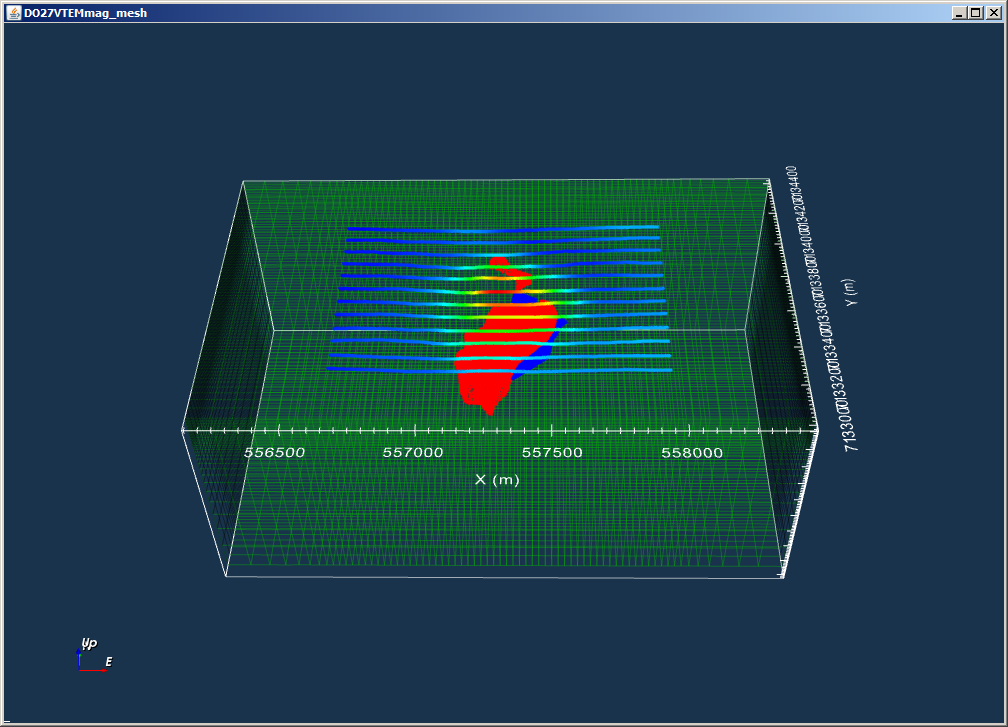
\includegraphics[width=0.8\textwidth]{images/TKC/TKCdataPKHK.PNG}
   \caption{Mesh used in this chapter along VTEM data, and outer bound of PK (red) and HK (blue)}
   \label{fig:TKCdataPKHK}
\end{figure}
%
Using the geology unit data sets and a geological model is created \autoref{fig:TKCgeoModel}. Given this geology model and using a parametric voxel inversion (this will be described in an earlier chapter) we now have a susceptibility model that closely matches know geological structure and makes an attempt at fitting the data \autoref{fig:TKCgeoModel}. 

% For this parametric inversion result the PK unit has an effective susceptibility of .00657(SI) and the HK unit has an effective susceptibility of .0271 (SI). These numbers may seem high but it is important to note that they are effect susceptibilities and not susceptibilities. Accounting for Koenigsberger ratios of HK and PK samples from TKC the results roughly fit petrophysical measurements. The fit of this synthetic model to the true data is shown in  \autoref{fig:paramModMisfitNorm}, the effective $\Phi_d$ of the predicted data is 
%
\begin{figure} [h]
   \centering
   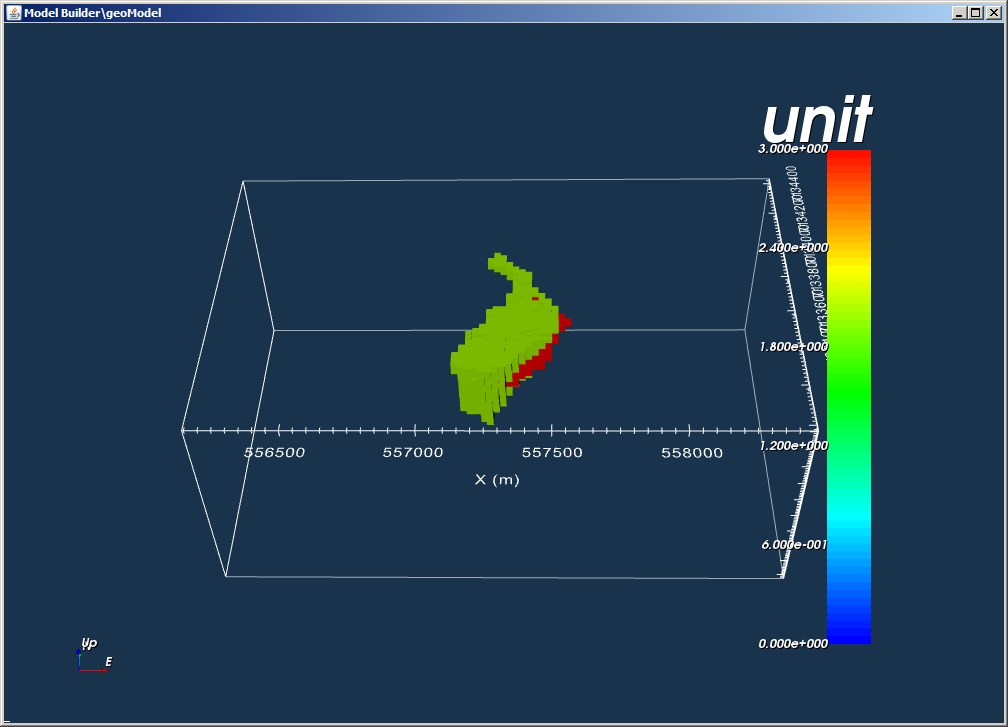
\includegraphics[width=0.8\textwidth]{images/TKC/TKCgeoModel.PNG}
   \caption{Geology model defined by geology data sets}
   \label{fig:TKCgeoModel}
\end{figure}

\begin{figure} [h]
   \centering
   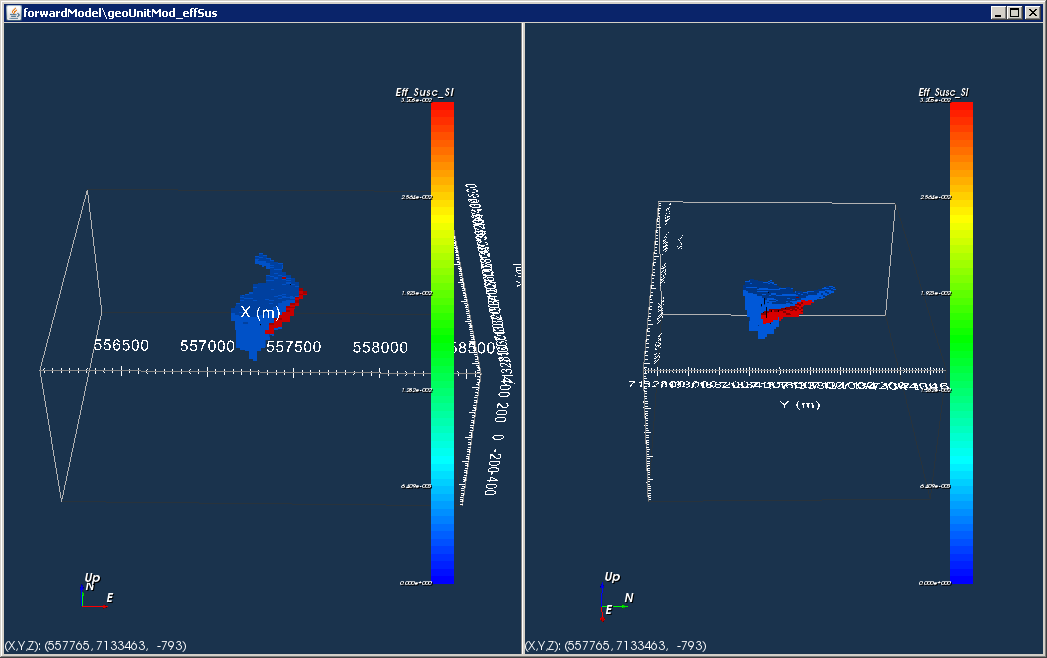
\includegraphics[width=0.8\textwidth]{images/TKC/TKCsuscModel.PNG}
   \caption{Geology model defined by geology data sets}
   \label{fig:TKCsuscModel}
\end{figure}

\begin{figure} [h]
   \centering
   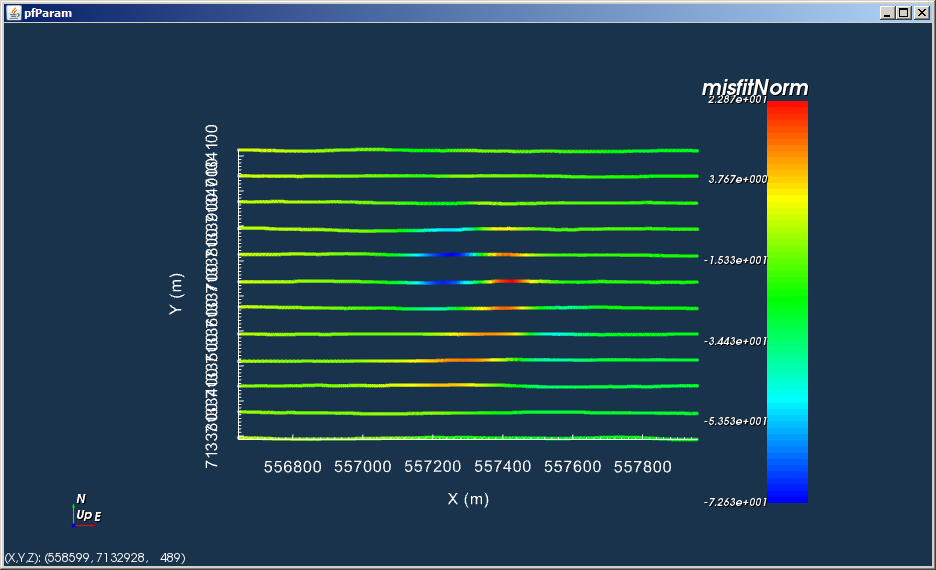
\includegraphics[width=0.8\textwidth]{images/TKC/paramModMisfitNorm.PNG}
   \caption{Normalized misfit of parametric voxel inversion}
   \label{fig:paramModMisfitNorm}
\end{figure}

\FloatBarrier
\section{Blind Inversion of the Synthetic Model}
\label{sec:Blind Inversion of the Synthetic Model:TKC}

%Show results. show how model is insufficiently compact and over estimates the amount of kimberlite

\section{Determination of Magnetization Dirrection}
\label{sec:Determination of Magnetization Dirrection}
%
%Correlation of Vertical and Total Gradients of Half RTP field \cite{dannemiller2006MagDirection}
%
%taking core direction from MVI result 
%
%apply recovered direction to the anomaly direction in MAG3D
%could also use parametric inversion and MVI sensitivities to provide more constraint.
%
%could apply anomalous dirrection locally to anomaly 
%
%In any case the result will be very similar to the earth's field in the location

\section{Creation of Constraints and Types of Data}
\label{sec:Creation of Constraints:TKC}

%Extensive Boreholes with rock units
%Multiple cross sections (crreated from said bore holes)
%Multiple data types to cluster



\subsection{$\alpha$ coefficients}
\label{sec:alpha coefficients:TKC}

%not much with alphas to be done here given that we don't expect discontinuity in any one particular dirrection.

\subsection{Reference Models}
%\label{sec:Reference Models:TKC}
%
%Most work to be done here. 
%
%We can create a reference model from the phys prop results from the borehole data. Perhaps we should only use some of the boreholes so that we have a more realistic amount of information than in a fully drilled example. We have two ways of applying phys prop measures to inversion and might use both. Also using $K_n$s to improve degree of fit between phys prop measures and effective susc recovered properties
%(show reference model)
%(show result)
%
%with sufficient boreholes we could make a incorrect surface that approximates the ``true'' model used. Use this with parametric inversion for reference model
%(show reference model)
%(show result)
%
%using clustering between density and mag (and conductivity and chargeablity) to create clusters, populate each cluster with a value either the mean value of the cluster or a parametric inversion and use as reference
%(show reference model)
%(show result)
%
%use cross section from \cite{harder2006geologyTKC}
%perhaps extend away from line and down weight
%(show reference model)
%(show result)
%
%(show Combined result)

\subsection{Weighting matrices}
\label{sec:Weighting matrices:TKC}
%
%smallness: using some measure of confidence in the measures decrease in cells with reference model specified to force the result to approximate the reference model. In case the cross section is extended down I will lower the $W_s$ as model cells are further away from the cross section
%(show smallness weight model)
%(show result, compare to result without)
%
%smoothness: to spread the model values away from where they are specified I can increase the smoothness weights in the vicinity of cells with specified reference models. 
%(show face weight model)
%
%with sufficient boreholes we could make a incorrect surface that approximates the ``true'' model used. Use this with parametric inversion for reference mode,l put lower weights along this surface.
%(show face weight model)
%
%using clustering between density and mag (and conductivity and chargeablity) to create clusters, populate each cluster with a value either the mean value of the cluster or a parametric inversion and use as reference
%(show result)
%
%(show result, compare to result without)
%
%(show Combined result)
\subsection{Bounds}
\label{sec:Bounds:TKC}
%
%Also useful for forcing model values to be near the specified reference model while allowing for uncertainty in our phys prop value. Since we have more statistical info on the 
%(show result)
%
%Need to determine if showing the field example is worthwhile at this point and how to bring it into the narrative

\endinput

Any text after an \endinput is ignored.
You could put scraps here or things in progress.

%
%    3. Notes
%    4. Footnotes

%    5. Bibliography
\begin{singlespace}
\raggedright
\bibliography{biblio}
\bibliographystyle{seg}
\end{singlespace}

\appendix
%    6. Appendices (including copies of all required UBC Research
%       Ethics Board's Certificates of Approval)
%\include{reb-coa}	% pdfpages is useful here
\chapter{Supporting Materials}

\begin{itemize}
\item
\end{itemize}


\backmatter
%    7. Index
% See the makeindex package: the following page provides a quick overview
% <http://www.image.ufl.edu/help/latex/latex_indexes.shtml>


\end{document}
